\documentclass[acmsmall]{acmart} % option for camera-ready differs from submission

 % following code block was received after completing the copyright form:
\setcopyright{cc}
\setcctype{by}
\acmJournal{PACMMOD}
\acmYear{2025}
\acmVolume{3}
\acmNumber{3 (SIGMOD)}
\acmArticle{221}
\acmMonth{6}
% \acmPrice{} % obsolete according to warning
\acmDOI{10.1145/3725358}

\usepackage[linesnumbered,ruled,vlined]{algorithm2e} % pseudo-code
%\usepackage{amsmath} % mathematical symbols; already loaded by ACM template
%\usepackage{amssymb} % mathematical symbols; should not be loaded because symbols already provided by ACM template (via "newtxmath")
%\usepackage{amsthm} % theorems, definitions etc.; already loaded by ACM template
%\usepackage{booktabs} % nicely formatted tables (with top, mid, and bottom rule); already loaded by ACM template
\usepackage{enumitem} % customized enumerations
%\usepackage{graphicx} % plots; already loaded by ACM template
\usepackage{multirow} % cells spanning multiple rows in tables
\usepackage{subcaption} % figures with multiple sub-figures and sub-captions
%\usepackage{hyperref} % links and URLs; already loaded by ACM template

% theorem environments also exist in ACM template by default, but use section numbering
\theoremstyle{acmplain}
\newtheorem{proposition}{Proposition}
\theoremstyle{acmdefinition}
\newtheorem{definition}{Definition}

\begin{document}

\title{Subgroup Discovery with Small and Alternative Feature Sets}

\author{Jakob Bach}
\orcid{0000-0003-0301-2798}
\affiliation{%
	\institution{Karlsruhe Institute of Technology (KIT)}
	\city{Karlsruhe}
	\country{Germany}
}
\email{jakob.bach@kit.edu}

% \renewcommand{\shortauthors}{Bach et al.} % for page headers if overlapping text

\begin{abstract}
Subgroup-discovery methods find interesting regions in a dataset.
In this article, we analyze two constraint types to enhance the interpretability of subgroups:
First, we make subgroup descriptions small by limiting the number of features used.
Second, we propose the novel problem of finding alternative subgroup descriptions, which cover a similar set of data objects as a given subgroup but use different features.
We describe how to integrate both constraint types into heuristic subgroup-discovery methods as well as a novel Satisfiability Modulo Theories (SMT) formulation, which enables a solver-based search for subgroups.
Further, we prove $\mathcal{NP}$-hardness of optimization with either constraint type.
Finally, we evaluate unconstrained and constrained subgroup discovery with 27 binary-classification datasets.
We observe that heuristic search methods often yield high-quality subgroups fast, even with constraints.
\end{abstract}

% The code below is generated by the tool at http://dl.acm.org/ccs.cfm
\begin{CCSXML}
	<ccs2012>
	<concept>
	<concept_id>10003752.10003809.10003716.10011141</concept_id>
	<concept_desc>Theory of computation~Mixed discrete-continuous optimization</concept_desc>
	<concept_significance>500</concept_significance>
	</concept>
	<concept>
	<concept_id>10010147.10010257.10010321.10010336</concept_id>
	<concept_desc>Computing methodologies~Feature selection</concept_desc>
	<concept_significance>500</concept_significance>
	</concept>
	<concept>
	<concept_id>10010147.10010257.10010258.10010259</concept_id>
	<concept_desc>Computing methodologies~Supervised learning</concept_desc>
	<concept_significance>300</concept_significance>
	</concept>
	<concept>
	<concept_id>10003752.10003777.10003779</concept_id>
	<concept_desc>Theory of computation~Problems, reductions and completeness</concept_desc>
	<concept_significance>300</concept_significance>
	</concept>
	</ccs2012>
\end{CCSXML}

\ccsdesc[500]{Theory of computation~Mixed discrete-continuous optimization}
\ccsdesc[500]{Computing methodologies~Feature selection}
\ccsdesc[300]{Computing methodologies~Supervised learning}
\ccsdesc[300]{Theory of computation~Problems, reductions and completeness}

\keywords{Subgroup Discovery, Constraints, Feature Selection, Alternatives, Satisfiability Modulo Theories, Explainability, Interpretability, XAI}

\received{October 2024} % dates specific to V3mod118 till V3mod236
\received[revised]{January 2025}
\received[accepted]{February 2025}

\maketitle

\section{Introduction}
\label{sec:csd:introduction}

\paragraph{Motivation}

Interpretable machine learning has gained importance in recent years~\cite{carvalho2019machine, molnar2020interpretable}.
Some machine-learning models are simple enough to be intrinsically interpretable~\cite{carvalho2019machine}, e.g., subgroup descriptions.
Subgroup discovery aims to identify `interesting' subsets of a dataset~\cite{atzmueller2015subgroup}, such as data objects sharing a specific class label, that can be described by concise conditions on feature values.
Subgroup-discovery methods have recently been employed in various fields, such as chemistry~\cite{li2021subgroup}, database engineering~\cite{remil2021makes}, decision making~\cite{zuheros2023explainable}, medicine~\cite{esnault2020qfinder}, and social sciences~\cite{kiefer2022subgroup}.

Figure~\ref{fig:csd:exemplary-subgroup} displays an exemplary rectangle-shaped subgroup description for a two-dimensional, real-valued dataset with a binary prediction target.
This subgroup is defined by $(\mathit{Feature\_1} \in [3.0, 5.1]) \land (\mathit{Feature\_2} \in [1.0, 1.8])$ and contains a high share of data objects with $\mathit{Target} = 1$.
If such subgroup descriptions become too complex, their interpretability suffers~\cite{meeng2021real}.
Thus, imposing constraints on subgroup descriptions may foster their interpretability.

\begin{figure}[t]
	\centering
	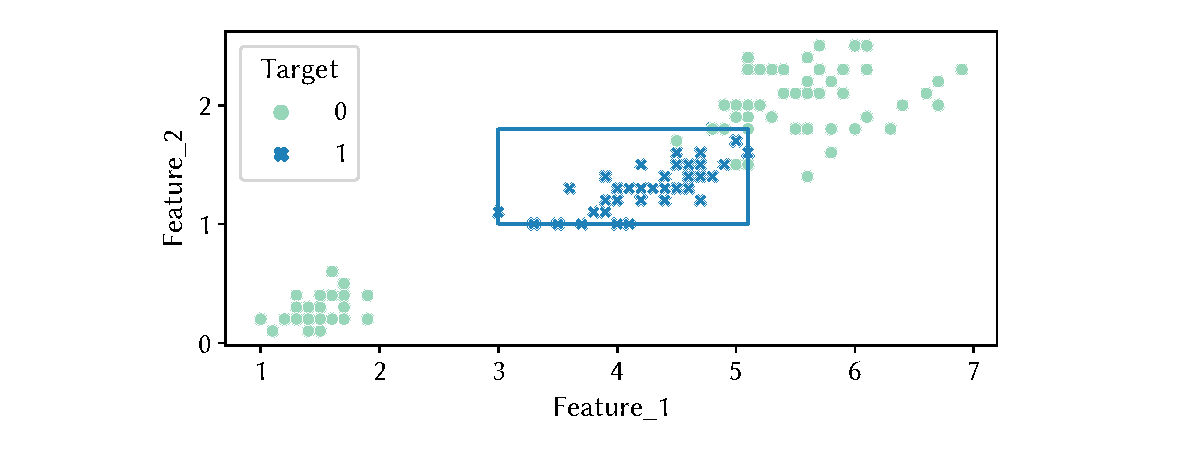
\includegraphics[width=\columnwidth, trim=15 15 15 14, clip]{plots/csd-exemplary-subgroup.pdf}
	\caption{
		Rectangular subgroup description for a dataset with two features and a binary prediction target.
	}
	\label{fig:csd:exemplary-subgroup}
\end{figure}

\paragraph{Problem statement}

This article addresses the problem of subgroup discovery with two types of constraints,
which both relate to the features used in subgroup descriptions:

First, \emph{feature-cardinality constraints} limit the number of selected, i.e., used, features.
Thus, subgroup descriptions become \emph{small}, which increases their interpretability for users at the potential expense of subgroup quality.
For example, in Figure~\ref{fig:csd:exemplary-subgroup}, a subgroup description may use either feature alone rather than both and still cover a high share of data objects with $\mathit{Target} = 1$.
Feature selection is common for other machine-learning tasks as well~\cite{guyon2003introduction, li2017feature}.

Second, \emph{alternative subgroup descriptions} should cover roughly the same set of data objects as a given subgroup but use different features.
For instance, in Figure~\ref{fig:csd:exemplary-subgroup}, one may define a subgroup based on one feature and then try to cover a similar set of data objects with bounds on the other feature.
Such alternative subgroup descriptions provide alternative explanations for the same subgroup.
Alternative explanations are also popular for other explainable-AI techniques like counterfactuals~\cite{mothilal2020explaining, russell2019efficient}, e.g., to enable users to develop and test several hypotheses or foster trust in the predictions~\cite{kim2021multi, wang2019designing}.
Consider subgroup discovery on scientific data, where a subgroup may capture samples exhibiting an interesting scientific phenomenon, and the subgroup description gives a possible explanation of which factors the phenomenon depends on.
Thus, users may leverage the subgroup description to formulate a scientific hypothesis for the domain.
Just considering one explanation may be misleading in such a situation.
For example, different factors (features) may explain the same phenomenon (subgroup), particularly if factors are correlated or interact with each other.
Thus, obtaining alternative subgroup descriptions may broaden the users' perspective and prevent selecting one explanation prematurely.

\paragraph{Related work}

Widely used subgroup-discovery methods are algorithmic~\cite{atzmueller2015subgroup, herrera2011overview}, so considering particular constraint types on subgroup descriptions usually entails type-specific adaptations.

The number of features used in a subgroup description is an established measure for subgroup complexity~\cite{helal2016subgroup, herrera2011overview, ventura2018subgroup}.
However, systematic evaluations of this constraint type are lacking, as existing work typically only analyzes one subgroup-discovery method or one cardinality threshold.

Various subgroup-discovery methods yield a set of diverse subgroups~\cite{belfodil2019fssd, bosc2018anytime, leeuwen2012diverse, lucas2018ssdp+}.
However, these alternative subgroups aim to cover different regions of the dataset rather than finding alternative descriptions for the same region.
Approaches that explicitly target alternative descriptions~\cite{boley2009non, galbrun2017redescription, lopez2023discovering, leeuwen2012diverse} are rarer and differ from our approach as well, as we discuss in Section~\ref{sec:csd:related-work}.

\paragraph{Contributions}

We make four main contributions:

(1) We formalize subgroup discovery as a Satisfiability Modulo Theories (SMT) optimization problem.
This novel white-box formulation admits a solver-based search for subgroups and allows integrating and combining constraints in a declarative manner.

(2) We formalize feature-cardinality constraints and the novel notion of alternative subgroup descriptions.
For the latter, we allow users to control the number and dissimilarity of alternatives.
We also describe how to integrate both constraint types into three existing heuristic subgroup-discovery methods and two novel baselines.

(3) We show that finding optimal solutions under these two constraint types is computationally hard by proving $\mathcal{NP}$-completeness.

(4) We conduct comprehensive experiments with 27 binary-classification datasets from the Penn Machine Learning Benchmarks (PMLB)~\cite{olson2017pmlb, romano2021pmlb} to compare solver-based and seven algorithmic search methods for subgroups, with and without constraints.
We publish all code\footnote{\url{https://github.com/Jakob-Bach/Constrained-Subgroup-Discovery}; additionally backed up in the \emph{Software Heritage archive} with the identifier \href{https://archive.softwareheritage.org/swh:1:dir:e587f3e572f07d879abae884f4a0c8aea8b0887d;origin=https://github.com/Jakob-Bach/Constrained-Subgroup-Discovery;visit=swh:1:snp:e2a212e43df12460d56ea557ee8f9470d3c3dcfb;anchor=swh:1:rev:8e8e1f5e54ac7644fc34f57cae2ad39b6fc1d453}{\texttt{swh:1:dir:e587f3e572f07d879abae884f4a0c8aea8b0887d}}} and experimental data\footnote{\url{https://doi.org/10.35097/nftgaf7w73hy2491}}.
We observe that two heuristic search methods yield similar subgroup quality as solver-based search while being one to two orders of magnitude faster.
Feature-cardinality constraints reduce overfitting, and a few features suffice to reach comparable subgroup quality as without constraints.
Finally, there may be multiple alternative subgroup descriptions with comparable quality and similarity to the original subgroup description.

\paragraph{Outline}

The remainder of this article is structured as follows:
Section~\ref{sec:csd:fundamentals} introduces fundamentals.
Section~\ref{sec:csd:baselines} proposes two baselines for subgroup discovery.
Section~\ref{sec:csd:approach} describes and analyzes constrained subgroup discovery.
Section~\ref{sec:csd:experimental-design} outlines our experimental design.
Section~\ref{sec:csd:evaluation} presents the corresponding experimental results.
Section~\ref{sec:csd:related-work} reviews related work.
Section~\ref{sec:csd:conclusion} concludes.

\section{Fundamentals}
\label{sec:csd:fundamentals}

In this section, we introduce relevant fundamentals of subgroup discovery:
the optimization problem (Section~\ref{sec:csd:fundamentals:problem}) and common algorithmic search methods (Section~\ref{sec:csd:fundamentals:search}).

\subsection{Problem of Subgroup Discovery}
\label{sec:csd:fundamentals:problem}

To harmonize formalization and evaluation, we focus on real-valued datasets with a binary prediction target.
$X \in \mathbb{R}^{m \times n}$ denotes a dataset in the form of a matrix.
Each row is a data object, and each column is a feature.
$y \in \{0, 1\}^m$ represents the binary prediction target.
Section~\ref{sec:csd:evaluation:summary-discussion} discusses adaptations for other scenarios.

For such real-valued datasets, a subgroup description typically forms a hyperrectangle in~$\mathbb{R}^n$ by defining a lower bound and an upper bound for each feature.
The bounds may also be infinite to leave a feature unrestricted.
A data object resides in the subgroup if all the data object's feature values satisfy the subgroup description's bounds:
%
\begin{definition}[Subgroup (description)]
	Given a dataset~$X \in \mathbb{R}^{m \times n}$, a \emph{subgroup} is described by its lower bounds~$\mathit{lb} \in \{\mathbb{R} \cup \{-\infty, +\infty\}\}^n$ and upper bounds~$\mathit{ub} \in \{\mathbb{R} \cup \{-\infty, +\infty\}\}^n$.
	Data object $X_{i \cdot}$ is a \emph{member} of this subgroup if $\forall j \in \{1, \dots, n\}:~ \left( X_{ij} \geq \mathit{lb}_j \right) \land \left( X_{ij} \leq \mathit{ub}_j \right)$.
	\label{def:csd:subgroup}
\end{definition}
%
To frame subgroup discovery as an optimization problem, let $Q(\mathit{lb}, \mathit{ub}, X, y)$ be the subgroup quality for a particular dataset:
%
\begin{definition}[Subgroup discovery]
	Given a dataset~$X \in \mathbb{R}^{m \times n}$ with prediction target $y \in \{0, 1\}^m$,
	\emph{subgroup discovery} is the problem of finding a subgroup (Definition~\ref{def:csd:subgroup}) with bounds~$\mathit{lb}, \mathit{ub} \in \{\mathbb{R} \cup \{-\infty, +\infty\}\}^n$ that maximizes a given notion of subgroup quality $Q(\mathit{lb}, \mathit{ub}, X, y)$.
	\label{def:csd:subgroup-discovery}
\end{definition}
%
For binary prediction targets, high-quality subgroups should typically contain many data objects from one class but few from the other.
Without loss of generality, we assume that the class with label~`1' is the class of interest, also called \emph{positive} class.
Weighted Relative Accuracy (WRAcc)~\cite{lavravc1999rule} is a popular metric for subgroup quality~\cite{meeng2021real}:
%
\begin{equation}
	\text{WRAcc} = \frac{m_b}{m} \cdot \left( \frac{m_b^+}{m_b} - \frac{m^+}{m} \right) = \frac{m_b^+}{m} - \frac{m_b \cdot m^+}{m^2}
	\label{eq:csd:wracc}
\end{equation}
%
Besides the total number of data objects~$m$, this metric considers the number of positive data objects~$m^+$, the number of subgroup members~$m_b$, and the number of positive subgroup members~$m_b^+$.
In particular, WRAcc is the product of two factors, i.e., the relative frequency of subgroup membership and the prevalence of the positive class in the subgroup compared to the whole dataset.

The maximum value of WRAcc depends on the frequencies of the two classes in the dataset.
Thus, it makes sense to normalize WRAcc when working with datasets with different class frequencies.
One option is a max-normalization to the range $[-1, 1]$~\cite{mathonat2021anytime}:
%
\begin{equation}
	\text{nWRAcc} = \frac{\text{WRAcc}}{\text{WRAcc}_{\text{max}}} = \frac{m_b^+ \cdot m - m^+ \cdot m_b}{m^+ \cdot (m - m^+)}
	\label{eq:csd:wracc-normalized}
\end{equation}

\subsection{Subgroup-Discovery Methods}
\label{sec:csd:fundamentals:search}

To discover subgroups, there are heuristic search methods, like PRIM~\cite{friedman1999bump} and Best Interval~\cite{mampaey2012efficient}, as well as exhaustive search methods, like SD-Map~\cite{atzmueller2009fast, atzmueller2006sd}, MergeSD~\cite{grosskreutz2009subgroup}, and BSD~\cite{lemmerich2016fast, lemmerich2010fast}.
In this section, we discuss five search methods that are relevant for our experiments; see~\cite{atzmueller2015subgroup, helal2016subgroup, herrera2011overview, ventura2018subgroup} for comprehensive surveys of subgroup discovery.

\paragraph{Patient Rule Induction Method (PRIM)}

\emph{PRIM}~\cite{friedman1999bump} consists of a peeling phase, which iteratively restricts the subgroup's bounds, and a pasting phase, which iteratively expands them.
In this article, we only use the peeling phase since pasting may have little effect on subgroup quality and is often left out~\cite{arzamasov2021reds}.
Peeling starts with a subgroup containing all data objects.
Each iteration excludes a fraction~$\alpha \in (0, 1)$ of data objects from the subgroup by setting a corresponding lower or upper bound on a feature.
Having tested two new bounds for each feature, the algorithm uses the subgroup with the highest quality for the next iteration.
Once the current subgroup contains at most a fraction~$\beta_0 \in [0, 1]$ of data objects, \emph{PRIM} returns the best subgroup from all iterations.

\paragraph{Beam Search (Beam)}

Beam search is a generic search strategy that is common in subgroup discovery as well~\cite{atzmueller2015subgroup}.
It maintains a set of currently best solution candidates, whose number is the beam width~$w \in \mathbb{N}$.
\emph{Beam} starts with $w$ unrestricted subgroup descriptions.
Each iteration tries to refine each solution candidate by updating either the lower or upper bound of one feature.
In contrast to \emph{PRIM}, all unique feature values in the subgroup may serve as new bounds.
The new beam comprises the highest-quality $w$~subgroups from the updates and the previous iteration.
Once the beam remains unchanged, the best of its subgroups is returned.

\paragraph{Best Interval (BI)}

\emph{BI}~\cite{mampaey2012efficient} is a subgroup-refinement procedure based on theoretical properties of the quality metric WRAcc (Equation~\ref{eq:csd:wracc}).
It can be used within a beam-search strategy.
Unlike \emph{Beam}, \emph{BI} updates a feature's lower and upper bounds simultaneously rather than separately but still requires only one pass over the feature's values to find the best update option.

\paragraph{SD-Map}

\emph{SD-Map}~\cite{atzmueller2006sd} is an exhaustive search method based on the pattern-mining algorithm \emph{FP-growth}~\cite{han2000mining}.
It assumes that numeric features are discretized and produces equality conditions of the form $X_{ij} = v$ instead of the numeric intervals we focus on (Definition~\ref{def:csd:subgroup}).
The extension \emph{SD-Map*}~\cite{atzmueller2009fast} adds support for numeric targets and quality-based pruning of the search space.

\paragraph{Bitset-based Subgroup Discovery (BSD)}

\emph{BSD}~\cite{lemmerich2010fast} is another exhaustive search method that produces equality conditions in the subgroup description.
It combines a branch-and-bound strategy with a special binary data representation and pruning techniques to speed up the search.
\emph{NumBSD}~\cite{lemmerich2016fast} can handle numeric targets, though the features are still assumed to be discrete.

\section{Baselines and Preliminaries}
\label{sec:csd:baselines}

In this section, we propose two \emph{baselines} for subgroup discovery, \emph{Random} (Section~\ref{sec:csd:baselines:random}) and \emph{MORS} (Section~\ref{sec:csd:baselines:mors}).
They are conceptually simpler than the heuristic search methods from Section~\ref{sec:csd:fundamentals:search} and serve as additional reference points in our experiments.
Section~\ref{sec:csd:baselines:mors} also lays essential groundwork for our complexity analyses in Sections~\ref{sec:csd:approach:cardinality:complexity} and~\ref{sec:csd:approach:alternatives:complexity}.

\begin{algorithm}[t]
	\DontPrintSemicolon
	\KwIn{Dataset~$X \in \mathbb{R}^{m \times n}$, \newline
		Prediction target~$y \in \{0, 1\}^m$, \newline
		Subgroup-quality function~$Q(\mathit{lb}, \mathit{ub}, X, y)$, \newline
		Number of iterations~$\mathit{n\_iters} \in \mathbb{N}$
	}
	\KwOut{Subgroup bounds~$\mathit{lb}, \mathit{ub} \in \{\mathbb{R} \cup \{-\infty, +\infty\}\}^n$}
	\BlankLine
	$Q^{\text{opt}} \leftarrow - \infty$\;
	\For{$\mathit{iters} \leftarrow 1$ \KwTo $\mathit{n\_iters}$}{
		\For{$j \leftarrow 1$ \KwTo $n$}{ \label{al:csd:random-search:line:sampling-start}
			$(\mathit{lb}_j,~ \mathit{ub}_j) \leftarrow (-\infty, +\infty)$\;
		}
		\For{$j \in$ get\_permissible\_feature\_idxs(\dots)}{ \label{al:csd:random-search:line:permissible-features}
			$(\mathit{lb}_j,~\mathit{ub}_j) \leftarrow$ sample\_uniformly(unique($X_{\cdot j}$)) \label{al:csd:random-search:line:sampling-end}
		}
		\If{$Q(\mathit{lb}, \mathit{ub}, X, y) > Q^{\text{opt}}$}{ \label{al:csd:random-search:line:optimum-update-start}
			$Q^{\text{opt}} \leftarrow Q(\mathit{lb}, \mathit{ub}, X, y)$\;
			$(\mathit{lb}^{\text{opt}},~ \mathit{ub}^{\text{opt}}) \leftarrow (\mathit{lb},~ \mathit{ub})$\; \label{al:csd:random-search:line:optimum-update-end}
		}
	}
	\For{$j \leftarrow 1$ \KwTo $n$}{ \label{al:csd:random-search:line:bounds-infty-start}
		\lIf{$\mathit{lb}_j^{\text{opt}} = \min_{i \in \{1, \dots, m\}} X_{ij}$}{$\mathit{lb}_j^{\text{opt}} \leftarrow -\infty$} 
		\lIf{$\mathit{ub}_j^{\text{opt}} = \max_{i \in \{1, \dots, m\}} X_{ij}$}{$\mathit{ub}_j^{\text{opt}} \leftarrow +\infty$} \label{al:csd:random-search:line:bounds-infty-end}
	}
	\Return{$\mathit{lb}^{\text{opt}},~ \mathit{ub}^{\text{opt}}$}
	\caption{\emph{Random Search} for subgroup discovery.}
	\label{al:csd:random-search}
\end{algorithm}

\subsection{Random}
\label{sec:csd:baselines:random}

The baseline \emph{Random} (Algorithm~\ref{al:csd:random-search}) generates and evaluates subgroups for a fixed number of iterations~$\mathit{n\_iters} \in \mathbb{N}$. 
In each iteration, this baseline randomly samples a lower bound and an upper bound for each feature, selecting these bounds uniformly from the feature's unique values (Lines~\ref{al:csd:random-search:line:sampling-start}--\ref{al:csd:random-search:line:sampling-end}).
To support feature-cardinality constraints, which we discuss later (Section~\ref{sec:csd:approach:cardinality}), the function \emph{get\_permissible\_feature\_idxs(\dots)} (Line~\ref{al:csd:random-search:line:permissible-features}) can restrict which features may be bounded; by default, all features are permissible.
Further, bounds become infinite if they do not exclude any data objects from the subgroup (Lines~\ref{al:csd:random-search:line:bounds-infty-start}--\ref{al:csd:random-search:line:bounds-infty-end}).
The algorithm tracks the best subgroup generated so far over the iterations (Lines~\ref{al:csd:random-search:line:optimum-update-start}--\ref{al:csd:random-search:line:optimum-update-end}) and finally returns it.

\begin{algorithm}[t]
	\DontPrintSemicolon
	\KwIn{Dataset~$X \in \mathbb{R}^{m \times n}$, \newline
		Prediction target~$y \in \{0, 1\}^m$
	}
	\KwOut{Subgroup bounds~$\mathit{lb}, \mathit{ub} \in \{\mathbb{R} \cup \{-\infty, +\infty\}\}^n$}
	\BlankLine
	\For{$j \leftarrow 1$ \KwTo $n$}{
		$\mathit{lb}_j \leftarrow \min\limits_{\substack{i \in \{1, \dots, m\} \\ y_i = 1}} X_{ij}$\; \label{al:csd:mors:line:bounds-start}
		$\mathit{ub}_j \leftarrow \max\limits_{\substack{i \in \{1, \dots, m\} \\ y_i = 1}} X_{ij}$\; \label{al:csd:mors:line:bounds-end}
		\lIf{$\mathit{lb}_j = \min_{i \in \{1, \dots, m\}} X_{ij}$}{$\mathit{lb}_j \leftarrow -\infty$} \label{al:csd:mors:line:bounds-infty-start}
		\lIf{$\mathit{ub}_j = \max_{i \in \{1, \dots, m\}} X_{ij}$}{$\mathit{ub}_j \leftarrow + \infty$} \label{al:csd:mors:line:bounds-infty-end}
	}
	\For{$j \notin \text{get\_permissible\_feature\_idxs(\dots)}$}{ \label{al:csd:mors:line:reset-start} \label{al:csd:mors:line:permissible-features}
		$(\mathit{lb}_j,~ \mathit{ub}_j) \leftarrow (-\infty, +\infty)$\; \label{al:csd:mors:line:reset-end}
	}
	\Return{$\mathit{lb}, \mathit{ub}$}
	\caption{\emph{MORS} for subgroup discovery.}
	\label{al:csd:mors}
\end{algorithm}

\subsection{Minimal Optimal-Recall Subgroup (MORS)}
\label{sec:csd:baselines:mors}

This baseline builds on the following definition:
%
\begin{definition}[Minimal Optimal-Recall Subgroup (MORS)]
	Given a dataset $X \in \mathbb{R}^{m \times n}$ with prediction target~$y \in \{0, 1\}^m$,
	the \emph{Minimal Optimal-Recall Subgroup (MORS)} is the subgroup (Definition~\ref{def:csd:subgroup}) whose lower and upper bounds of each feature correspond to the minimum and maximum value of that feature over all positive data objects (i.e., with $y_i = 1$) from the dataset~$X$.
	\label{def:csd:mors}
\end{definition}
%
The definition ensures that all positive data objects are subgroup members.
Thus, the evaluation metric \emph{recall}, i.e., the fraction of positive data objects becoming subgroup members, reaches its \emph{optimal} value of~1.
At the same time, raising the lower bounds or lowering the upper bounds would exclude positive data objects from the subgroup.
In this sense, the set of subgroup members is \emph{minimal}.
The corresponding subgroup description is unique and solves the following variant of the subgroup-discovery problem:
%
\begin{definition}[Minimal-optimal-recall-subgroup discovery]
	Given a dataset $X \in \mathbb{R}^{m \times n}$ with prediction target~$y \in \{0, 1\}^m$,
	\emph{minimal-optimal-recall-subgroup discovery} is the problem of finding a subgroup (Definition~\ref{def:csd:subgroup}) that contains as few negative data objects (i.e., with $y_i = 0$) as possible but all positive data objects (i.e., with $y_i = 1$) from the dataset~$X$.
	\label{def:csd:minimal-optimal-recall-subgroup-discovery}
\end{definition}
%
I.e., the problem aims to minimize the number of false positives subject to producing no false negatives.
Equivalently, it maximizes the number of true negatives, i.e., negative data objects excluded from the subgroup, subject to producing no false negatives.

Algorithm~\ref{al:csd:mors} implements the baseline (Lines~\ref{al:csd:mors:line:bounds-start}--\ref{al:csd:mors:line:bounds-end}), followed by adaptations for feature-cardinality constraints (Lines~\ref{al:csd:mors:line:bounds-infty-start}--\ref{al:csd:mors:line:reset-end}).
Since \emph{MORS} only needs to iterate over all data objects and features once to determine the minimum and maximum feature values, its time complexity is~$O(m \cdot n)$.
This places minimal-optimal-recall-subgroup discovery in the complexity class~$\mathcal{P}$:
%
\begin{proposition}[Complexity for Definition~\ref{def:csd:minimal-optimal-recall-subgroup-discovery}]
	The problem of minimal-optimal-recall-subgroup discovery (Definition~\ref{def:csd:minimal-optimal-recall-subgroup-discovery}) can be solved in~$O(m \cdot n)$.
	\label{prop:csd:complexity-unconstrained-minimal-optimal-recall-subgroup-discovery}
\end{proposition}
%
Interestingly, a kind of inverted problem definition, the \textsc{Maximum Box} problem, is $\mathcal{NP}$-hard~\cite{eckstein2002maximum}.
The latter problem maximizes the number of true positives, i.e., positive data objects in the subgroup, subject to producing no false positives, thereby retaining an optimal precision of~1.

For later proofs, we also need the following concept~\cite{meeng2014rocsearch}:
%
\begin{definition}[Perfect subgroup]
	Given a dataset~$X \in \mathbb{R}^{m \times n}$ with prediction target~$y \in \{0, 1\}^m$,
	a \emph{perfect subgroup} is a subgroup (Definition~\ref{def:csd:subgroup}) that contains all positive data objects (i.e., with $y_i = 1$) but no negative data objects (i.e., with $y_i = 0$) from the dataset~$X$.
	\label{def:csd:perfect-subgroup}
\end{definition}
%
Perfect subgroups reach the maximum possible WRAcc (Equation~\ref{eq:csd:wracc}) for a dataset.
Next, we define a corresponding search problem:
%
\begin{definition}[Perfect-subgroup discovery]
	Given a dataset~$X \in \mathbb{R}^{m \times n}$ with prediction target~$y \in \{0, 1\}^m$,
	\emph{perfect-subgroup discovery} is the problem of finding a perfect subgroup (Definition~\ref{def:csd:perfect-subgroup}) if it exists or determining that it does not exist.
	\label{def:csd:perfect-subgroup-discovery}
\end{definition}
%
This problem is easy to solve with the help of Algorithm~\ref{al:csd:mors}.
In particular, after \emph{MORS} has found a subgroup in~$O(m \cdot n)$, one only needs to check whether the subgroup contains any negative data objects.
If it does not, the subgroup is perfect, otherwise no perfect subgroup exists.
In particular, the \emph{MORS} bounds cannot be tightened to exclude negative data objects without also excluding positives, thereby violating the perfection of the subgroup.
Thus, we obtain the following result: 
%
\begin{proposition}[Complexity for Definition~\ref{def:csd:perfect-subgroup-discovery}]
	The problem of perfect-subgroup discovery (Definition~\ref{def:csd:perfect-subgroup-discovery}) can be solved in~$O(m \cdot n)$.
	\label{prop:csd:complexity-unconstrained-perfect-subgroup}
\end{proposition}

\section{Constrained Subgroup Discovery}
\label{sec:csd:approach}

In this section, we propose an SMT encoding of subgroup discovery (Section~\ref{sec:csd:approach:smt}) and discuss feature-cardinality constraints (Section~\ref{sec:csd:approach:cardinality}) as well as alternative subgroup descriptions (Section~\ref{sec:csd:approach:alternatives}).

\subsection{SMT Encoding of Subgroup Discovery}
\label{sec:csd:approach:smt}

Encoding subgroup discovery as a white-box optimization problem enables a solver-based search for subgroups.
Such a formulation supports integrating constraints declaratively, while algorithmic search methods need specific adaptations for constraints.
Here, we propose a Satisfiability Modulo Theories (SMT) encoding.
SMT generally allows expressions in first-order logic with particular interpretations, e.g., arrays, arithmetic, or bit vectors~\cite{barrett2018satisfiability}.
Here, we use linear real arithmetic (LRA).
The mixture of logical and arithmetic expressions in SMT makes it relatively straightforward to express subgroup discovery and the two constraint types we analyze.
In preliminary experiments, we also considered an encoding as a mixed-integer linear program, but the latter formulation required more decision variables and constraints, and optimization was slower.

We define decision variables $\mathit{lb}, \mathit{ub} \in \{\mathbb{R} \cup \{-\infty, +\infty\}\}^n$ for the bounds of the subgroup description (Definition~\ref{def:csd:subgroup}).
The upper bounds naturally need to be at least as high as the lower bounds:
%
\begin{equation}
	\forall j \in \{1, \dots, n\}:~ \mathit{lb}_j\leq \mathit{ub}_j
	\label{eq:csd:smt-constraint-bounds-monotonic}
\end{equation}
%
Next, we introduce binary decision variables~$b_i \in \{0, 1\}^m$ for subgroup membership.
A data object is a member of the subgroup if all its feature values are contained within the bounds (Definition~\ref{def:csd:subgroup}):
%
\begin{equation}
	\forall i \in \{1, \dots, m\}:~ b_i\leftrightarrow \bigwedge_{j \in \{1, \dots, n\}} \left( \left( X_{ij} \geq \mathit{lb}_j \right) \land \left( X_{ij} \leq \mathit{ub}_j \right) \right)
	\label{eq:csd:smt-constraint-subgroup-membership}
\end{equation}
%
Finally, we encode WRAcc (Equation~\ref{eq:csd:wracc}) as the objective function.
$m_b$ and $m_b^+$ depend on the decision variables~$b_i$ while $m$ and $m^+$ are dataset-dependent constants.
Thus, WRAcc is linear in~$b_i$:
%
\begin{equation}
	\max \quad Q_{\text{WRAcc}} = \frac{1}{m} \cdot \sum_{\substack{i \in \{1, \dots, m\} \\ y_i = 1 }} b_i - \frac{m^+}{m^2} \cdot \sum_{i=1}^{m} b_i \\
	\label{eq:csd:smt-wracc}
\end{equation}
%
Instead of introducing the decision variables~$b_i$, one could also insert the Boolean expression on the right-hand side of Equation~\ref{eq:csd:smt-constraint-subgroup-membership} into Equation~\ref{eq:csd:smt-wracc} directly.
In particular, $\mathit{lb}_j$ and $\mathit{ub}_j$ are the only decision variables strictly necessary for the optimization problem.
However, we also use the variables~$b_i$ for encoding alternative subgroup descriptions later and therefore make them explicit.

\subsection{Feature-Cardinality Constraints}
\label{sec:csd:approach:cardinality}

In this section, we discuss feature-cardinality constraints for subgroup discovery.
First, we motivate and define them (Section~\ref{sec:csd:approach:cardinality:concept}).
Next, we describe how to integrate them into our SMT encoding (Section~\ref{sec:csd:approach:cardinality:smt}), heuristic search methods (Section~\ref{sec:csd:approach:cardinality:heuristics}), and baselines (Section~\ref{sec:csd:approach:cardinality:baselines}).
Finally, we analyze the time complexity of subgroup discovery with this constraint type (Section~\ref{sec:csd:approach:cardinality:complexity}).

\subsubsection{Concept}
\label{sec:csd:approach:cardinality:concept}

Complex subgroup descriptions may be hard to interpret~\cite{meeng2021real}.
Feature-cardinality constraints simplify subgroup descriptions by limiting the number of features used in them.
In particular, we define feature selection for subgroups as follows:
%
\begin{definition}[Feature selection in subgroups]
	Given a dataset~$X \in \mathbb{R}^{m \times n}$ and a subgroup (Definition~\ref{def:csd:subgroup}) with bounds~$\mathit{lb}, \mathit{ub} \in \{\mathbb{R} \cup \{-\infty, +\infty\}\}^n$,
	Feature~$j$ is \emph{selected} if the bounds exclude at least one data object of~$X$ from the subgroup, i.e., $\exists i \in \{1, \dots, m\}: \left( X_{ij} < \mathit{lb}_j \right) \lor \left( X_{ij} > \mathit{ub}_j \right)$.
	\label{def:csd:feature-selection}
\end{definition}
%
The bounds of unselected features can be considered infinite, effectively removing them from the subgroup description.
The \emph{feature cardinality} of a subgroup description is the number of selected features, sometimes called the description's \emph{length} in the literature~\cite{atzmueller2015subgroup, helal2016subgroup}.
A feature-cardinality constraint imposes an upper bound on the number of selected features:
%
\begin{definition}[Feature-cardinality constraint]
	Given a cardinality threshold $k \in \mathbb{N}$,
	a \emph{feature-cardinality constraint} for a subgroup (Definition~\ref{def:csd:subgroup}) requires the subgroup to have at most $k$~features selected (Definition~\ref{def:csd:feature-selection}).
	\label{def:csd:feature-cardinality-constraint}
\end{definition}
%
A subgroup-discovery method may also select less than $k$~features if selecting more does not improve subgroup quality.

\subsubsection{SMT Encoding}
\label{sec:csd:approach:cardinality:smt}

To encode whether a feature is selected or not, we introduce binary decision variables $s, s^{\text{lb}}, s^{\text{ub}} \in \{0, 1\}^n$.
Based on Definition~\ref{def:csd:feature-selection}, a feature is selected if its minimum is less than the lower bound or its maximum is greater than the upper bound:
%
\begin{equation}
	\begin{aligned}
		\forall j \in \{1, \dots, n\}: & & s^{\text{lb}}_j &\leftrightarrow \left( \mathit{lb}_j > \min_{i \in \{1, \dots, m\}} X_{ij} \right) \\
		\forall j \in \{1, \dots, n\}: & &s^{\text{ub}}_j &\leftrightarrow \left( \mathit{ub}_j < \max_{i \in \{1, \dots, m\}} X_{ij} \right) \\
		\forall j \in \{1, \dots, n\}: & & s_j &\leftrightarrow \left( s^{\text{lb}}_j \lor s^{\text{ub}}_j \right)
	\end{aligned}
	\label{eq:csd:smt-constraint-feature-selection}
\end{equation}
%
Minimum and maximum feature values are constants that can be determined before formulating the optimization problem.

Given the variables~$s_j$ (Equation~\ref{eq:csd:smt-constraint-feature-selection}), setting an upper bound on the number of selected features (Definition~\ref{def:csd:feature-cardinality-constraint}) is straightforward:
%
\begin{equation}
	\sum_{j=1}^n s_j \leq k
	\label{eq:csd:smt-constraint-feature-cardinalty}
\end{equation}
%
Instead of defining the decision variables $s_j$, $s^{\text{lb}}_j$, and $s^{\text{ub}}_j$, one could also insert the corresponding expressions from Equation~\ref{eq:csd:smt-constraint-feature-selection} into Equation~\ref{eq:csd:smt-constraint-feature-cardinalty} directly.

\subsubsection{Integration into Heuristic Search Methods (Section~\ref{sec:csd:fundamentals:search})}
\label{sec:csd:approach:cardinality:heuristics}

The feature-cardinality constraint (Equation~\ref{eq:csd:smt-constraint-feature-cardinalty}) has the form~$|F_s| \leq k$ for the feature set~$F_s$ induced by the selection decisions~$s \in \{0, 1\}^n$.
Thus, the constraint is \emph{antimonotonic}~\cite{ng1998exploratory} regarding the set of selected features.
In particular, the empty feature set satisfies the constraint for any~$k \geq 0$.
If a set of selected features satisfies the constraint, all its subsets also satisfy it.
Vice versa, if a feature set violates the constraint, all its supersets violate it as well.

The antimonotonicity property eases integrating the constraint into \emph{Beam}, \emph{BI}, and \emph{PRIM}.
These three methods iteratively enlarge the set of selected features.
In particular, they start with unrestricted subgroup bounds, i.e., an empty feature set.
Each iteration may either add bounds on one further feature, thereby increasing the feature-set size by one, or refine the bounds on an already selected feature, so the feature-set size remains constant.
Features cannot be deselected, so the feature-set size is non-decreasing overall.
Once $k$~features are selected, we only allow bounds on these features to be refined.
Due to antimonotonicity, all potential feature supersets are invalid anyway.
In contrast, any feature may be bounded as long as fewer than $k$~features are selected.

\subsubsection{Integration into Baselines (Section~\ref{sec:csd:baselines})}
\label{sec:csd:approach:cardinality:baselines}

For \emph{Random}, we sample~$k$ out of $n$~features uniformly random without replacement.
This step implements the function \emph{get\_permissible\_feature\_idxs(\dots)} in Line~\ref{al:csd:random-search:line:permissible-features} of Algorithm~\ref{al:csd:random-search}.
Next, we sample these features' bounds as usual.
For \emph{MORS}, we employ a univariate, quality-based heuristic for feature selection in Line~\ref{al:csd:mors:line:permissible-features} of Algorithm~\ref{al:csd:mors}:
For each feature, we determine the number of negative data objects in the subgroup if only this feature uses \emph{MORS} bounds.
We select the $k$~features with the lowest number of false positives.
This heuristic is equivalent to selecting the features with the highest WRAcc for univariate \emph{MORS} bounds.

\subsubsection{Computational Complexity}
\label{sec:csd:approach:cardinality:complexity}

Without constraints, an exhaustive search for subgroups needs to evaluate $O(m^{2n})$ subgroup descriptions.
In particular, each feature has $O(m)$ unique values, resulting in $O(m^2)$ relevant lower-upper-bound combinations that are combined over $n$~features.
Thus, the number of features impacts the search space exponentially, while the number 
of data objects has a polynomial impact.
In practice, this expression only is an upper bound:
Exhaustive search methods may employ quality-based pruning to not evaluate all solution candidates explicitly~\cite{atzmueller2015subgroup}.

With a feature-cardinality constraint, there are $\binom{n}{k} \leq n^k$ feature sets of size~$k$ with $O(m^{2k})$ bound candidates each, resulting in $O(n^k \cdot m^{2k})$ candidate subgroup descriptions.
This complexity term is exponential in the number of selected features~$k$.
However, for a fixed~$k$, the term is polynomial in the dataset size~$m \cdot n$.
Thus, the problem is in the parameterized complexity class $\mathcal{XP}$~\cite{downey1997parameterized}:
%
\begin{proposition}[Parameterized complexity for Definition~\ref{def:csd:subgroup-discovery} with~\ref{def:csd:feature-cardinality-constraint}]
	The problem of subgroup discovery (Definition~\ref{def:csd:subgroup-discovery}) with a feature-cardinality constraint (Definition~\ref{def:csd:feature-cardinality-constraint}) resides in the parameterized complexity class~$\mathcal{XP}$ for the parameter~$k$.
	\label{prop:csd:complexity-cardinality-xp}
\end{proposition}
%
Without a feature-cardinality constraint, $\mathcal{XP}$ membership holds for the parameter~$n$ instead of~$k$.

\cite{boley2009non} showed that it is an $\mathcal{NP}$-hard problem to find a subgroup description minimizing feature cardinality while inducing exactly the same subgroup membership as a given subgroup description.
We adapt this hardness result to optimizing subgroup quality under a feature-cardinality constraint.
First, we tackle the search problem for perfect subgroups:
%
\begin{proposition}[Complexity for Definition~\ref{def:csd:perfect-subgroup-discovery} with~\ref{def:csd:feature-cardinality-constraint}]
	The problem of perfect-subgroup discovery (Definition~\ref{def:csd:perfect-subgroup-discovery}) with a feature-cardinality constraint (Definition~\ref{def:csd:feature-cardinality-constraint}) is $\mathcal{NP}$-complete.
	\label{prop:csd:complexity-cardinality-np-perfect-subgroup}
\end{proposition}
%
\begin{proof}
	Let~$I$ be an arbitrary instance of the decision problem \textsc{Set Covering}~\cite{karp1972reducibility}.
	$I$ consists of a set of elements~$E = \{e_1, \dots, e_m\}$, a set of sets~$\mathbb{S} = \{S_1, \dots, S_n\}$ with $E = \bigcup_{S \in \mathbb{S}} S$, and a cardinality~$k \in \mathbb{N}$.
	\textsc{Set Covering} asks whether a subset $\mathbb{C} \subseteq \mathbb{S}$ exists with $|\mathbb{C}| \leq k$ and $E = \bigcup_{S \in \mathbb{C}} S$, i.e., containing each element from~$E$ in at least one set and consisting of at most $k$~sets.
	
	We transform~$I$ into an instance~$I'$ of the perfect-subgroup-discovery problem with a feature-cardinality constraint (Definitions~\ref{def:csd:perfect-subgroup-discovery} and~\ref{def:csd:feature-cardinality-constraint}).
	First, we keep the cardinality threshold~$k \in \mathbb{N}$.
	Next, we define the dataset~$X \in \{0, 1\}^{(m + 1) \times n}$ such that $X_{ij}$ encodes $e_i \in S_j$, i.e., membership of Element~$i$ in Set~$j$.
	The index $i = m + 1$ represents a \emph{dummy element} that is not part of any set, so all its feature values are set to~0.
	Finally, we define the prediction target~$y \in \{0, 1\}^{m+1}$ as $y_{m+1} = 1$ and $y_i = 0$ otherwise.
	$y$~represents whether an element should \emph{not} be covered by~$\mathbb{C} \subseteq \mathbb{S}$.
	In particular, all elements from~$E$ should be covered but not the dummy element.
	
	A perfect subgroup (Definition~\ref{def:csd:perfect-subgroup}) exactly replicates the prediction target as subgroup membership.
	Hence, with our definition of~$X$ and~$y$ for problem instance~$I'$, a perfect subgroup only contains the data object representing the dummy element.
	As all feature values of this dummy data object are~0, the subgroup description only consists of the bounds $\mathit{lb}_j = \mathit{ub}_j = 0$ for selected features.
	Thus, the data objects excluded from the subgroup assume the value~1 for at least one selected feature.
	I.e., all elements from~$E$ are in a selected set, so the selected features represent a set cover~$\mathbb{C}$.

	In contrast, if no feature set of the desired size~$k$ can describe a perfect subgroup, then always at least one data object with~$y_i = 0$ has to be in the subgroup.
	Thus, at least one element from~$E$ must not be in any selected set, so no valid set cover of size~$k$ exists.
	
	Overall, a solution to the instance~$I'$ of the perfect-subgroup-discovery problem with a feature-cardinality constraint also solves the instance~$I$ of \textsc{Set Covering}.
	Since the latter problem is $\mathcal{NP}$-hard~\cite{karp1972reducibility}, the former is as well.
	To be more precise, our problem is $\mathcal{NP}$-complete since checking a solution only entails a polynomial cost of~$O(m \cdot n)$, requiring one pass over the dataset to determine subgroup membership and feature selection.
\end{proof}
%
This hardness result contrasts with the polynomial runtime of unconstrained perfect-subgroup discovery (Proposition~\ref{prop:csd:complexity-unconstrained-perfect-subgroup}), which corresponds to a cardinality constraint with $k = n$.

Generalizing Proposition~\ref{prop:csd:complexity-cardinality-np-perfect-subgroup}, the optimization problem of subgroup discovery with a feature-cardinality constraint is $\mathcal{NP}$-complete under a reasonable assumption regarding subgroup quality:
%
\begin{proposition}[Complexity for Definition~\ref{def:csd:subgroup-discovery} with~\ref{def:csd:feature-cardinality-constraint}]
	Assuming a subgroup-quality function~$Q(\mathit{lb}, \mathit{ub}, X, y)$ for which only perfect subgroups (Definition~\ref{def:csd:perfect-subgroup}) reach its maximal value,
	the problem of subgroup discovery (Definition~\ref{def:csd:subgroup-discovery}) with a feature-cardinality constraint (Definition~\ref{def:csd:feature-cardinality-constraint}) is $\mathcal{NP}$-complete.
	\label{prop:csd:complexity-cardinality-np}
\end{proposition}
%
\begin{proof}
	Let~$I$ be an arbitrary instance of the perfect-subgroup-discovery problem with a feature-cardinality constraint (Definitions~\ref{def:csd:perfect-subgroup-discovery} and~\ref{def:csd:feature-cardinality-constraint}).
	We transform~$I$ into an instance~$I'$ of the subgroup-discovery problem (Definition~\ref{def:csd:subgroup-discovery}) with a feature-cardinality constraint.
	In particular, we optimize a subgroup-quality function $Q(\mathit{lb}, \mathit{ub}, X, y)$ rather than searching for a perfect subgroup (Definition~\ref{def:csd:perfect-subgroup}).
	The other problem inputs remain the same.
	
	Based on the assumption on~$Q(\mathit{lb}, \mathit{ub}, X, y)$ in Proposition~\ref{prop:csd:complexity-cardinality-np}, the solution for~$I'$ is a perfect subgroup if the latter exists.
	Thus, if the optimal subgroup for~$I'$ is not perfect, then a perfect subgroup does not exist.
	Checking whether a subgroup is perfect entails a cost of $O(m \cdot n)$.
	Overall, an algorithm for subgroup discovery with a feature-cardinality constraint solves perfect-subgroup discovery with a feature-cardinality constraint with negligible overhead.
	Since the latter problem is $\mathcal{NP}$-complete (Proposition~\ref{prop:csd:complexity-cardinality-np-perfect-subgroup}) and the former resides in $\mathcal{NP}$, the former is also $\mathcal{NP}$-complete.
\end{proof}
%
WRAcc (Equation~\ref{eq:csd:wracc}) satisfies the assumption of Proposition~\ref{prop:csd:complexity-cardinality-np} since only perfect subgroups, i.e., with $m_b^+ = m_b = m^+$, yield the theoretical maximum WRAcc.

\subsection{Alternative Subgroup Descriptions}
\label{sec:csd:approach:alternatives}

In this section, we propose the optimization problem of discovering alternative subgroup descriptions.
First, we motivate and formalize the problem (Section~\ref{sec:csd:approach:alternatives:concept}).
Next, we describe how to phrase it within our SMT encoding (Section~\ref{sec:csd:approach:alternatives:smt}), heuristic search methods (Section~\ref{sec:csd:approach:alternatives:heuristics}), and baselines (Section~\ref{sec:csd:approach:alternatives:baselines}).
Finally, we analyze the time complexity of this problem (Section~\ref{sec:csd:approach:alternatives:complexity}).

\subsubsection{Concept}
\label{sec:csd:approach:alternatives:concept}

We assume to have an \emph{original subgroup} given, which may originate from any subgroup-discovery method.
In a nutshell, alternative subgroup descriptions should induce similar subgroup membership of data objects as the original subgroup but select different features.
One can search multiple such alternative descriptions sequentially. 
In this case, alternative descriptions should also select different features than all previous alternatives.
We count the original subgroup as the zeroth alternative.
Formally, we define the optimization problem as follows:
%
\begin{definition}[Alternative-subgroup-description discovery]
	Given
	\begin{itemize}[noitemsep]
		\item a dataset $X \in \mathbb{R}^{m \times n}$,
		\item $a \in \mathbb{N}$ existing subgroups with subgroup membership~$b^{(l)} \in \{0, 1\}^m$ and feature selection~$s^{(l)} \in \{0, 1\}^n$ for $l \in \{0, \dots, a - 1\}$,
		\item a similarity measure $\text{sim}(\cdot)$ for subgroup-membership vectors,
		\item a dissimilarity measure $\text{dis}(\cdot)$ for feature-selection vectors of subgroups,
		\item and a dissimilarity threshold~$\tau \in \mathbb{R}_{\geq 0}$,
	\end{itemize}
	\emph{alternative-subgroup-description discovery} is the problem of finding a subgroup (Definition~\ref{def:csd:subgroup}) with membership~$b^{(a)} \in \{0, 1\}^m$ and feature selection~$s^{(a)} \in \{0, 1\}^n$ that maximizes the subgroup-membership similarity $\text{sim}(b^{(a)}, b^{(0)})$ to the original subgroup while being dissimilar to all existing subgroups regarding the feature selection, i.e., $\forall l \in \{0, \dots, a-1\}:~\text{dis}(s^{(a)}, s^{(l)}) \geq \tau$.
	\label{def:csd:alternative-subgroup-description-discovery}
\end{definition}
%
Users can control the number of alternatives~$a \in \mathbb{N}$ and the dissimilarity threshold~$\tau \in \mathbb{R}_{\geq 0}$.
Due to the sequential search procedure that yields alternatives one by one, users can stop the search after each alternative.
Further, we recommend employing a feature-cardinality constraint (Definition~\ref{def:csd:feature-cardinality-constraint}) so subgroup descriptions are easier to interpret and sufficiently many features are left for alternatives.
Next, we discuss our choice of $\text{sim}(\cdot)$ and $\text{dis}(\cdot)$.

\paragraph{Similarity in objective function}

Various options exist to quantify the similarity between two binary subgroup-membership vectors $b', b'' \in \{0, 1\}^m$.
We turn the Hamming distance~\cite{choi2010survey} into a similarity measure and normalize it to $[0, 1]$ with the vector lengths, obtaining the following \emph{normalized Hamming similarity}:
%
\begin{equation}
	\text{sim}_{\text{nHamm}}(b', b'') = \frac{1}{m} \cdot \sum_{i=1}^{m} (b'_i = b''_i)
	\label{eq:csd:hamming-general}
\end{equation}
%
If either $b'$ or $b''$ is constant, this similarity measure is linear in its remaining argument (Equation~\ref{eq:csd:smt-hamming}).
Further, if one considers one vector to be a prediction and the other to be the ground truth, Equation~\ref{eq:csd:hamming-general} equals prediction accuracy for binary classification.

Another popular similarity measure for sets or binary vectors is the Jaccard index~\cite{choi2010survey}, which relates the overlap of positive vector entries to their union:
%
\begin{equation}
	\text{sim}_{\text{Jacc}}(b', b'') = \frac{\sum_{i=1}^{m} (b'_i \land b''_i)}{\sum_{i=1}^{m} (b'_i \lor b''_i)}
	\label{eq:csd:jaccard}
\end{equation}
%
However, this similarity measure is not linear in~$b'$ and~$b''$, which limits its applicability in some white-box solvers. 
Thus, we opt for the normalized Hamming similarity as the objective function.

\paragraph{Dissimilarity in constraints}

There are various options to quantify the dissimilarity between feature-selection vectors.
We formulate a constraint with the following \emph{deselection dissimilarity}:
%
\begin{equation}
	\text{dis}_{\text{des}}(s^{\text{new}}, s^{\text{old}}) = \sum_{j=1}^n (\lnot s^{\text{new}}_j \land s^{\text{old}}_j) \geq \min \left( \tau_{\text{abs}},~k^{\text{old}} \right)
	\label{eq:csd:constraint-dissimilarity}
\end{equation}
%
This dissimilarity counts how many previously selected features are \emph{not} selected in the new subgroup description, either being replaced by other features or the total number of selected features being reduced.
A valid solution must deselect at least $\tau_{\text{abs}} \in \mathbb{N}$ features unless the number selected before ($k^{\text{old}}$) is smaller, in which case all these must be deselected.
For maximum dissimilarity, none of the previously selected features may be selected again.
This dissimilarity measure is asymmetric, i.e., $\text{dis}_{\text{des}}(s^{\text{new}}, s^{\text{old}}) \neq \text{dis}_{\text{des}}(s^{\text{old}}, s^{\text{new}})$.
However, `old' and `new' are well-defined in sequential search for alternatives.
We explicitly designed our deselection dissimilarity to satisfy two desirable properties, which common dissimilarity measures like the Jaccard distance or the Dice dissimilarity~\cite{choi2010survey} violate:
(1)~If $s^{\text{old}}$ is constant, Equation~\ref{eq:csd:constraint-dissimilarity} is linear in $s^{\text{new}}$, even if the exact number of newly selected features is unknown yet.
This property is useful for solver-based search.
(2)~Equation~\ref{eq:csd:constraint-dissimilarity} is antimonotonic in the new feature selection, which is useful for heuristic search.

\subsubsection{SMT Encoding}
\label{sec:csd:approach:alternatives:smt}

Reformulating Equation~\ref{eq:csd:hamming-general}, we see that the objective is linear regarding the alternative membership vector~$b^{(a)}$:
%
\begin{equation}
	\begin{aligned}
		\text{sim}_{\text{nHamm}}(b^{(a)}, b^{(0)}) &= \frac{1}{m} \cdot \sum_{i=1}^m \left( b_i^{(a)} \leftrightarrow b_i^{(0)} \right) \\
		&= \frac{1}{m} \cdot \Big( \sum\limits_{\substack{i \in \{1, \dots, m\} \\ b_i^{(0)} = 1}} b_i^{(a)} + \sum\limits_{\substack{i \in \{1, \dots, m\} \\ b_i^{(0)} = 0}} \lnot b_i^{(a)} \Big)
	\end{aligned}
	\label{eq:csd:smt-hamming}
\end{equation}
%
In particular, since $b^{(0)}$~is known and therefore constant, we employ the expression from the second line, involving two plain sums.
The negation~$\lnot b_i^{(a)}$ may also be expressed as $1 - b_i^{(a)}$.

To formulate the dissimilarity constraints, we leverage that the feature-selection vector~$s^{(l)}$ and the corresponding number of selected features~$k^{(l)}$ are known for all existing subgroups as well.
Thus, we instantiate and adapt Equation~\ref{eq:csd:constraint-dissimilarity} as follows:
%
\begin{equation}
	\forall l \in \{0, \dots, a-1\}:~ \text{dis}_{\text{des}}(s^{(a)}, s^{(l)}) = \sum_{\substack{j \in \{1, \dots, n\} \\ s^{(l)}_j = 1}} \lnot s^{(a)}_j \geq \min \left( \tau_{\text{abs}},~k^{(l)} \right)
	\label{eq:csd:smt-constraint-dissimilarity}
\end{equation}
%
In particular, we only sum over features that were selected in the $l$-th existing subgroup and check whether they are deselected now.

\subsubsection{Integration into Heuristic Search Methods (Section~\ref{sec:csd:fundamentals:search})}
\label{sec:csd:approach:alternatives:heuristics}

The situation resembles integrating a feature-cardinality constraint (Section~\ref{sec:csd:approach:cardinality:heuristics}).
In particular, since the dissimilarity constraint (Equation~\ref{eq:csd:constraint-dissimilarity}) is antimonotonic in the subgroup's feature selection, the constraint is suitable for heuristic search methods that iteratively enlarge the set of selected features.
In each iteration, we only need to check how many previously selected features are selected again.
In particular, once $k^{(l)} - \tau_{\text{abs}}$~features from an existing subgroup description with $k^{(l)}$~features are selected, no additional features from this subgroup may be selected for defining bounds.

\subsubsection{Integration into Baselines (Section~\ref{sec:csd:baselines})}
\label{sec:csd:approach:alternatives:baselines}

Adapting our two baselines to alternative subgroup descriptions is not straightforward since the optimization objective changes, and the search space under the dissimilarity constraint (Equation~\ref{eq:csd:constraint-dissimilarity}) is more complex.
Thus, we did not implement and evaluate concrete adaptations.
In particular, \emph{MORS} is tailored towards a particular notion of subgroup quality, i.e., recall, instead of optimizing subgroup-membership similarity.
For \emph{Random}, we would like to uniformly sample from a constrained search space, which is a hard problem in general~\cite{ermon2012uniform}.
We could also sample from the unconstrained space until a valid feature set is found, which may take a long time.
Another option is non-uniform sampling, e.g., only sample features not selected in any existing subgroup, which ignores the permitted feature-set overlap.

\subsubsection{Computational Complexity}
\label{sec:csd:approach:alternatives:complexity}

The size of the search space for alternative subgroup descriptions is comparable to that of discovering original subgroups, i.e., exponential in the number of features.
The main difference is that the dissimilarity constraint needs to be considered.
We prove $\mathcal{NP}$-completeness for a special case of alternative-subgroup-description discovery (Definition~\ref{def:csd:alternative-subgroup-description-discovery}) first.
To this end, we introduce the following definition:
%
\begin{definition}[Perfect alternative subgroup description]
	Given
	\begin{itemize}[noitemsep]
		\item a dataset $X \in \mathbb{R}^{m \times n}$,
		\item an original subgroup with subgroup membership~$b^{(0)} \in \{0, 1\}^m$ and feature selection~$s^{(0)} \in \{0, 1\}^n$,
		\item a dissimilarity measure $\text{dis}(\cdot)$ for feature-selection vectors of subgroups,
		\item and a dissimilarity threshold~$\tau \in \mathbb{R}_{\geq 0}$,
	\end{itemize}
	a \emph{perfect alternative subgroup description} defines a subgroup (Definition~\ref{def:csd:subgroup}) with membership~$b^{(a)} \in \{0, 1\}^m$ and feature selection~$s^{(a)} \in \{0, 1\}^n$ that exactly replicates the subgroup membership of the original subgroup, i.e., $b^{(a)} = b^{(0)}$, while being dissimilar regarding the feature selection, i.e., $\text{dis}(s^{(a)}, s^{(0)}) \geq \tau$.
	\label{def:csd:perfect-alternative}
\end{definition}
%
In particular, the value of the subgroup-membership similarity is fixed rather than an optimization objective.
Similar to perfect subgroups (Definition~\ref{def:csd:perfect-subgroup}), perfect alternative subgroup descriptions only exist in some datasets. 
We now define a corresponding search problem:
%
\begin{definition}[Perfect-alternative-subgroup-description discovery]
	Given
	\begin{itemize}[noitemsep]
		\item a dataset $X \in \mathbb{R}^{m \times n}$,
		\item an original subgroup with subgroup membership~$b^{(0)} \in \{0, 1\}^m$ and feature selection~$s^{(0)} \in \{0, 1\}^n$,
		\item a dissimilarity measure $\text{dis}(\cdot)$ for feature-selection vectors of subgroups,
		\item and a dissimilarity threshold~$\tau \in \mathbb{R}_{\geq 0}$,
	\end{itemize}
	\emph{perfect-alternative-subgroup-description discovery} is the problem of finding a perfect alternative subgroup description (Definition~\ref{def:csd:perfect-alternative}) if it exists or determining that it does not exist.
	\label{def:csd:perfect-alternative-subgroup-description-discovery}
\end{definition}
%
This search problem is $\mathcal{NP}$-complete under a reasonable assumption on the employed notion of feature-selection dissimilarity:
%
\begin{proposition}[Complexity for Definition~\ref{def:csd:perfect-alternative-subgroup-description-discovery} with~\ref{def:csd:feature-cardinality-constraint}]
	Assuming a combination of a dissimilarity measure~$\text{dis}(\cdot)$ and a dissimilarity threshold~$\tau \in \mathbb{R}_{\geq 0}$ that prevents selecting any selected feature from the original subgroup description again,
	the problem of perfect-alternative-subgroup-description discovery (Definition~\ref{def:csd:perfect-alternative-subgroup-description-discovery}) with a feature-cardinality constraint (Definition~\ref{def:csd:feature-cardinality-constraint}) is $\mathcal{NP}$-complete.
	\label{prop:csd:complexity-perfect-alternatives-np-perfect-subgroup}
\end{proposition}
%
Our deselection dissimilarity (Equation~\ref{eq:csd:constraint-dissimilarity}) as~$\text{dis}(\cdot)$ satisfies the assumption from Proposition~\ref{prop:csd:complexity-perfect-alternatives-np-perfect-subgroup} if we choose a dissimilarity threshold~$\tau_{\text{abs}} \geq k^{\text{old}}$, as in the following proof.
Other dissimilarity measures should typically also have a threshold value that enforces zero overlap between feature sets.
Additionally, the problem naturally remains $\mathcal{NP}$-complete when dropping the assumption.
%
\begin{proof}
	Let~$I$ be an arbitrary instance of the perfect-subgroup-discovery problem with a feature-cardinality constraint (Definitions~\ref{def:csd:perfect-subgroup-discovery} and~\ref{def:csd:feature-cardinality-constraint}).	
	We transform~$I$ into an instance~$I'$ of the perfect-alternative-subgroup-description-discovery problem (Definition~\ref{def:csd:perfect-alternative-subgroup-description-discovery}), also with a feature-cardinality constraint.
	First, we retain the feature-cardinality threshold~$k \in \mathbb{N}$.
	Next, we define the original subgroup for~$I'$ to be perfect (Definition~\ref{def:csd:perfect-subgroup}), i.e., having subgroup membership $b^{(0)} = y$.
	Further, we choose the deselection dissimilarity (Equation~\ref{eq:csd:constraint-dissimilarity}) as~$\text{dis}(\cdot)$ and set $\tau_{\text{abs}} = k$.
	In particular, no feature from the original subgroup description may be selected again.
	We define dataset~$X' \in \mathbb{R}^{m \times (n+k)}$ of problem instance~$I'$ as dataset~$X \in \mathbb{R}^{m \times n}$ of problem instance~$I$ with $k$~extra features that were all selected in the original subgroup description, i.e., $\forall j \in \{n+1, \dots, n+k\}:~ s^{(0)}_j = 1$ and $\forall j \in \{1, \dots, n\}:~s^{(0)}_j = 0$.
	For solving~$I'$, we need not explicitly define the $k$~extra features but could imagine them to equal the prediction target~$y$.
	
	A solution for problem instance~$I'$ also solves~$I$.
	In particular, the perfect alternative subgroup description (Definition~\ref{def:csd:perfect-alternative}) defines a perfect subgroup here since it perfectly replicates the original subgroup membership, which is perfect, i.e., $b^{(a)} = b^{(0)} = y$.
	Due to the dissimilarity constraint, the alternative subgroup description only selects features from the original dataset~$X$.
	Thus, if a perfect alternative subgroup description for~$I'$ exists, it also solves~$I$.
	If it does not exist, then there also is no other perfect subgroup for~$I$.

	Overall, an algorithm for perfect-alternative-subgroup-description discovery with a feature-cardinality constraint also solves perfect-subgroup discovery with a feature-cardinality constraint with negligible overhead.
	Since the latter problem is $\mathcal{NP}$-complete (Proposition~\ref{prop:csd:complexity-cardinality-np-perfect-subgroup}) and evaluating a solution for the former problem entails a polynomial cost, the former is $\mathcal{NP}$-complete as well.
\end{proof}

Next, we switch from the search problem for perfect alternatives to the optimization problem for alternative subgroup descriptions in general.
We establish $\mathcal{NP}$-completeness under a reasonable assumption on the employed notion of subgroup-membership similarity:
%
\begin{proposition}[Complexity for Definition~\ref{def:csd:alternative-subgroup-description-discovery} with~\ref{def:csd:feature-cardinality-constraint}]
	Assuming
	\begin{itemize}[noitemsep]
		\item a combination of a dissimilarity measure~$\text{dis}(\cdot)$ and a dissimilarity threshold~$\tau \in \mathbb{R}_{\geq 0}$ that prevents selecting any selected feature from the original subgroup description again,
		\item and a similarity measure~$\text{sim}(\cdot)$ for which only perfect alternative subgroup descriptions (Definition~\ref{def:csd:perfect-alternative}) reach its maximal value regarding the original subgroup,
	\end{itemize}
	the problem of alternative-subgroup-description discovery (Definition~\ref{def:csd:alternative-subgroup-description-discovery}) with a feature-cardinality constraint (Definition~\ref{def:csd:feature-cardinality-constraint}) is $\mathcal{NP}$-complete.
	\label{prop:csd:complexity-alternatives-np}
\end{proposition}
%
\begin{proof}
	Let~$I$ be an arbitrary instance of the perfect-alternative-subgroup-description-discovery problem with a feature-cardinality constraint (Definitions~\ref{def:csd:perfect-alternative-subgroup-description-discovery} and~\ref{def:csd:feature-cardinality-constraint}).
	We transform~$I$ into a problem instance~$I'$ of the alternative-subgroup-description-discovery problem (Definition~\ref{def:csd:alternative-subgroup-description-discovery}), also with a feature-cardinality constraint.
	In particular, we optimize subgroup-membership similarity~$\text{sim}(\cdot)$ rather than searching for a perfect alternative subgroup description (Definition~\ref{def:csd:perfect-alternative}).
	The other problem inputs remain the same.
	
	Based on the assumption we made on~$\text{sim}(\cdot)$ in Proposition~\ref{prop:csd:complexity-alternatives-np}, the optimal solution for~$I'$ is a perfect alternative subgroup description if the latter exists.
	Thus, if the optimal subgroup description for~$I'$ is not a perfect alternative, then the latter does not exist.
	Overall, an algorithm for alternative-subgroup-description discovery with a feature-cardinality constraint solves perfect-alternative-subgroup-description discovery with a feature-cardinality constraint with negligible overhead.
	Since the latter problem is $\mathcal{NP}$-complete (Proposition~\ref{prop:csd:complexity-perfect-alternatives-np-perfect-subgroup}) and the former problem resides in~$\mathcal{NP}$, the former is $\mathcal{NP}$-complete as well.
\end{proof}
%
Normalized Hamming similarity (Equation~\ref{eq:csd:hamming-general}) satisfies the $\text{sim}(\cdot)$ assumption from Proposition~\ref{prop:csd:complexity-alternatives-np} since only perfect alternative subgroup descriptions yield the theoretical maximum similarity of~1.

\section{Experimental Design}
\label{sec:csd:experimental-design}

In this section, we introduce our experimental design:
subgroup-discovery methods, experimental scenarios, evaluation metrics, datasets, and the implementation.

\paragraph{Subgroup-discovery methods}

We compare eight search methods for subgroup discovery:
three exhaustive ones and five heuristic ones.

As the exhaustive search method \emph{SMT}, we use the solver \emph{Z3}~\cite{bjorner2015nuz, deMoura2008z3} to tackle our SMT encoding (Section~\ref{sec:csd:approach:smt}).
We set solver timeouts to keep runtime under control.
The solver returns the optimal solution if found, otherwise the best solution so far. 
The actual runtime is higher than the timeout due to the initialization effort before optimization.
We evaluate twelve exponentially scaled timeout values, i.e., \{1~s, 2~s, 4~s, $\dots$, 2048~s\}.
The default value is 2048~s unless specified otherwise.

We also evaluate two exhaustive search methods from related work, i.e., \emph{BSD}~\cite{lemmerich2010fast} and \emph{SD-Map}~\cite{atzmueller2006sd}, based on their implementation in the package \emph{SD4Py}~\cite{hudson2023subgroup}.
Both methods require discretizing numeric features.
We use their built-in equal-width discretization and tune it by choosing the best subgroup quality out of ten bin counts. i.e., $\{2, 3, 4, 5, 10, 15, 20, 30, 40, 50\}$.

As heuristics, we employ three search methods from related work (Section~\ref{sec:csd:fundamentals:search}) and our two baselines (Section~\ref{sec:csd:baselines}).
For \emph{PRIM}, we set the peeling fraction to~$\alpha = 0.05$, consistent with other implementations~\cite{arzamasov2021reds, kwakkel2017exploratory} and the recommended value range proposed by its authors~\cite{friedman1999bump}.
We set the support threshold to~$\beta_0 = 0$, so there is no constraint on subgroup size.
For \emph{Beam} and \emph{BI}, we choose a beam width of $w=10$, falling between default values used in other implementations~\cite{arzamasov2021reds, lemmerich2019pysubgroup}.
For \emph{Random}, we set the number of iterations to~$\mathit{n\_iters} = 1000$.
\emph{MORS} is parameter-free.

\paragraph{Experimental scenarios}

First, we analyze feature-cardinality constraints (Section~\ref{sec:csd:approach:cardinality}) for all eight subgroup-discovery methods.
We evaluate $k \in \{1, 2, 3, 4, 5\}$ as upper bounds on the number of selected features and also compare to the unconstrained problem.
Since the exhaustive search methods \emph{BSD} and \emph{SD-Map} did not finish within two days in the unconstrained setting for five datasets, we replace these missing values with the results for $k=5$.

Second, we study alternative subgroup descriptions (Section~\ref{sec:csd:approach:alternatives}) for \emph{SMT} and \emph{Beam}, i.e., the solver-based and one heuristic search method.
We choose a small~$k=3$ to leave enough unused features for describing alternatives.
We search for $a=5$ alternative subgroup descriptions with a dissimilarity threshold $\tau_{\text{abs}} \in \{1, 2, 3\}$.

\paragraph{Evaluation metrics}

We use three types of evaluation metrics:

(1) We quantify \emph{subgroup quality} with \emph{nWRAcc} (Equation~\ref{eq:csd:wracc-normalized}).
We conduct a stratified five-fold cross-validation.
In particular, each run of a subgroup-discovery method uses only 80\% of the data objects of a dataset as the training set, while the rest serves as the test set.
Thus, we can investigate how well a subgroup description from the training set generalizes to data objects from the test set.

(2) We measure the \emph{runtime} of the subgroup-discovery methods.

(3) To assess \emph{subgroup similarity} of alternative subgroup descriptions, we use \emph{normalized Hamming similarity} (Equation~\ref{eq:csd:hamming-general}) and \emph{Jaccard similarity} (Equation~\ref{eq:csd:jaccard}) for subgroup membership.

\begin{table}[t]
	\centering
	\caption{
		Datasets from PMLB used in our experiments.
		$m$~denotes the number of data objects and $n$~the number of features.
	}
	\begin{tabular}{lrr}
		\toprule
		Dataset & $m$ & $n$ \\
		\midrule
		backache & 180 & 32 \\
		chess & 3196 & 36 \\
		churn & 5000 & 20 \\
		clean1 & 476 & 168 \\
		clean2 & 6598 & 168 \\
		coil2000 & 9822 & 85 \\
		credit\_g & 1000 & 20 \\
		dis & 3772 & 29 \\
		GAMETES\_Epistasis\_2\_Way\_20atts\_0.1H\_EDM\_1\_1 & 1600 & 20 \\
		GAMETES\_Epistasis\_2\_Way\_20atts\_0.4H\_EDM\_1\_1 & 1600 & 20 \\
		GAMETES\_Epistasis\_3\_Way\_20atts\_0.2H\_EDM\_1\_1 & 1600 & 20 \\
		GAMETES\_Heterogeneity\_20atts\_1600\_Het\_0.4\_0.2\_50\_EDM\_2\_001 & 1600 & 20 \\
		GAMETES\_Heterogeneity\_20atts\_1600\_Het\_0.4\_0.2\_75\_EDM\_2\_001 & 1600 & 20 \\
		Hill\_Valley\_with\_noise & 1212 & 100 \\
		horse\_colic & 368 & 22 \\
		hypothyroid & 3163 & 25 \\
		ionosphere & 351 & 34 \\
		molecular\_biology\_promoters & 106 & 57 \\
		mushroom & 8124 & 22 \\
		ring & 7400 & 20 \\
		sonar & 208 & 60 \\
		spambase & 4601 & 57 \\
		spect & 267 & 22 \\
		spectf & 349 & 44 \\
		tokyo1 & 959 & 44 \\
		twonorm & 7400 & 20 \\
		wdbc & 569 & 30 \\
		\bottomrule
	\end{tabular}
	\label{tab:csd:datasets}
\end{table}

\paragraph{Datasets}

We use binary-classification datasets from the Penn Machine Learning Benchmarks (PMLB)~\cite{olson2017pmlb, romano2021pmlb}.
In each dataset, we choose the less frequent class as the positive class.
To avoid scenarios that may be too easy or lack enough features for alternative subgroup descriptions, we exclude datasets with fewer than 100 data objects or fewer than 20 features.
Next, we exclude one dataset with 1000 features, which has significantly more features than all remaining datasets.
Finally, we manually exclude datasets that are duplicates of others.
In the end, we obtain 27 datasets with 106 to 9822 data objects and 20 to 168 features (Table~\ref{tab:csd:datasets}).
The datasets do not contain missing values, and categorical features are ordinally encoded by default.

\paragraph{Implementation}

We implemented our experiments in Python~3.8.
All code is available online (Section~\ref{sec:csd:introduction}).
We organized the subgroup-discovery methods and evaluation metrics as a Python package to ease reuse.
Our experimental pipeline parallelizes over datasets, cross-validation folds, and subgroup-discovery methods, while each of these experimental tasks runs single-threaded.
Executing the pipeline took about 34~hours on a server with 160~GB RAM and an \emph{AMD EPYC 7551} CPU with 32~cores and 2.0~GHz base clock.

\section{Evaluation}
\label{sec:csd:evaluation}

We evaluate feature-cardinality constraints first (Section~\ref{sec:csd:evaluation:cardinality}) and alternative subgroup descriptions second (Section~\ref{sec:csd:evaluation:alternatives}).
Finally, we summarize and discuss the experimental results (Section~\ref{sec:csd:evaluation:summary-discussion}).

\subsection{Feature-Cardinality Constraints}
\label{sec:csd:evaluation:cardinality}

\begin{figure}[t]
	\centering
	\begin{subfigure}[t]{0.48\textwidth}
		\centering
		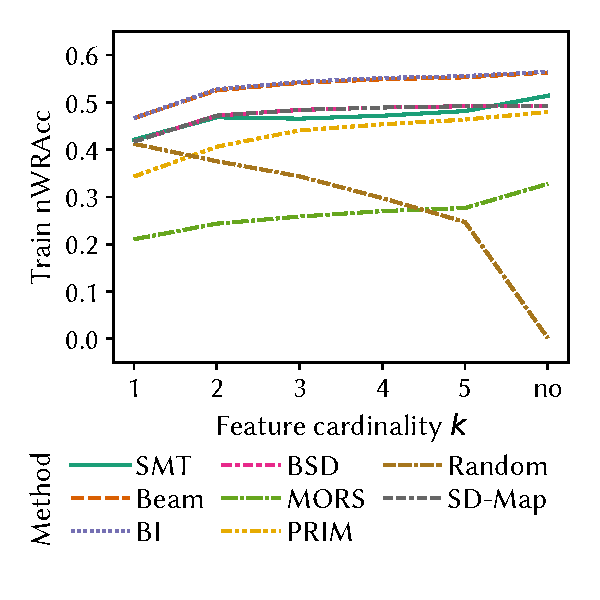
\includegraphics[width=\textwidth, trim=10 25 10 10, clip]{plots/csd-cardinality-train-nwracc-all-datasets.pdf}
		\caption{All 27 datasets, training set.}
		\label{fig:csd:cardinality-train-nwracc-all-datasets}
	\end{subfigure}
	\hfill
	\begin{subfigure}[t]{0.48\textwidth}
		\centering
		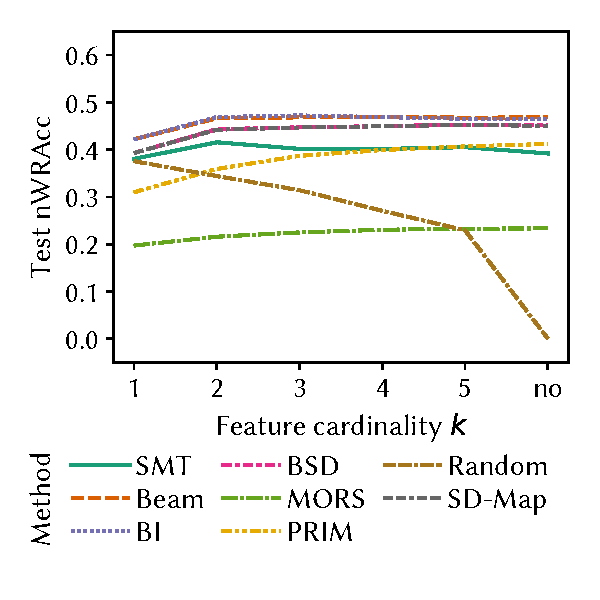
\includegraphics[width=\textwidth, trim=10 25 10 10, clip]{plots/csd-cardinality-test-nwracc-all-datasets.pdf}
		\caption{All 27 datasets, test set.}
		\label{fig:csd:cardinality-test-nwracc-all-datasets}
	\end{subfigure}
	\\ \vspace{\baselineskip}
	\begin{subfigure}[t]{0.48\textwidth}
		\centering
		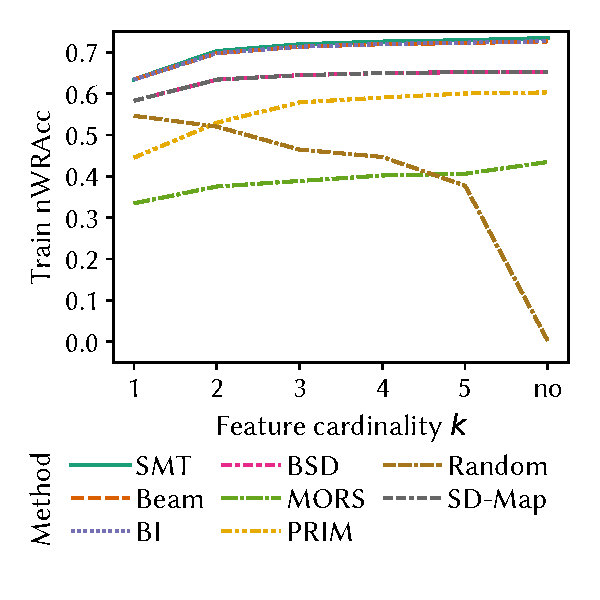
\includegraphics[width=\textwidth, trim=10 25 10 10, clip]{plots/csd-cardinality-train-nwracc-no-timeout-datasets.pdf}
		\caption{13 datasets without \emph{SMT} timeouts, training set.}
		\label{fig:csd:cardinality-train-nwracc-no-timeout-datasets}
	\end{subfigure}
	\hfill
	\begin{subfigure}[t]{0.48\textwidth}
		\centering
		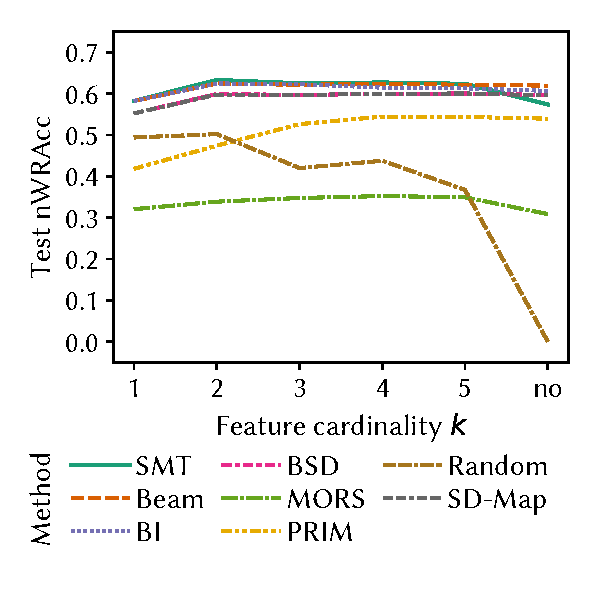
\includegraphics[width=\textwidth, trim=10 25 10 10, clip]{plots/csd-cardinality-test-nwracc-no-timeout-datasets.pdf}
		\caption{13 datasets without \emph{SMT} timeouts, test set.}
		\label{fig:csd:cardinality-test-nwracc-no-timeout-datasets}
	\end{subfigure}
	\caption{
		Mean subgroup quality over datasets and cross-validation folds, by subgroup-discovery method and feature cardinality~$k$.
		Results from the search for original subgroups.
	}
	\label{fig:csd:cardinality}
\end{figure}

\begin{figure}[t]
	\centering
	\begin{subfigure}[t]{0.48\textwidth}
		\centering
		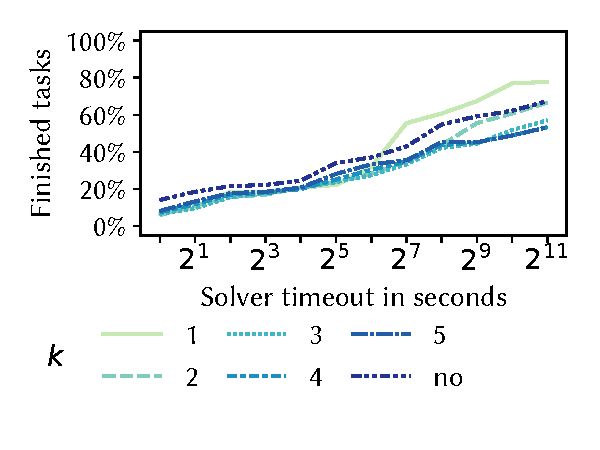
\includegraphics[width=\textwidth, trim=10 25 10 10, clip]{plots/csd-timeouts-finished-tasks.pdf}
		\caption{
			Frequency of finished \emph{SMT} tasks over datasets and cross-validation folds, by feature cardinality~$k$.
		}
		\label{fig:csd:timeouts-finished-tasks}
	\end{subfigure}
	\hfill
	\begin{subfigure}[t]{0.48\textwidth}
		\centering
		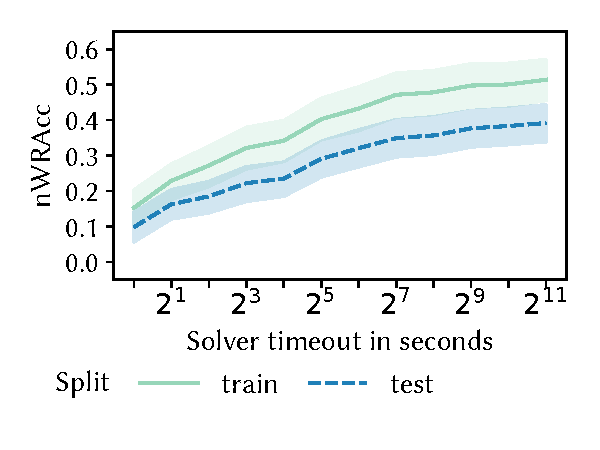
\includegraphics[width=\textwidth, trim=10 25 10 10, clip]{plots/csd-timeouts-nwracc.pdf}
		\caption{
			Mean subgroup quality, with 95\% confidence intervals based on datasets and cross-validation folds.
			Results without a feature-cardinality constraint.
		}
		\label{fig:csd:timeouts-nwracc}
	\end{subfigure}
	\caption{
		Impact of solver timeouts for \emph{SMT} as the subgroup-discovery method.
		Results from the search for original subgroups.
	}
	\label{fig:csd:timeouts}
\end{figure}

\paragraph{Training-set subgroup quality}

Figure~\ref{fig:csd:cardinality-train-nwracc-all-datasets} displays the training-set nWRAcc for subgroup-discovery methods and feature-cardinality thresholds~$k$, averaged over datasets and cross-validation folds.
The heuristic search methods \emph{Beam} and \emph{BI} are best on average and even outperform the solver-based search method \emph{SMT}.
This outcome is possible because \emph{SMT} may run into timeouts and then yield suboptimal results.
Figure~\ref{fig:csd:timeouts-finished-tasks} visualizes how many of the \emph{SMT} optimization tasks for original subgroups finished within the evaluated solver timeouts.
Additionally, Figure~\ref{fig:csd:timeouts-nwracc} shows how the mean subgroup quality of \emph{SMT} increases with higher solver-timeout settings.
For the maximum timeout setting of 2048~s and without a feature-cardinality constraint, 67.4\% of the \emph{SMT} searches finished, and 17 out of 27 datasets did not encounter timeouts.
However, even if we limit our evaluation to the datasets without solver timeouts (Figure~\ref{fig:csd:cardinality-train-nwracc-no-timeout-datasets}), \emph{Beam} and \emph{BI} are still remarkably close to the optimum quality.
Note that this result is not specific to our method \emph{SMT} but highlights a strong competition for any other exhaustive search method.

\emph{BSD} and \emph{SD-Map} yield worse average subgroup quality than \emph{Beam} and \emph{BI} as well.
While the former two theoretically are exhaustive, they require discretization of numeric features.
Thus, they effectively only have a fixed set of intervals to use as bounds instead of being able to choose the bounds independently at each possible feature value.
\emph{PRIM}'s worse subgroup quality may equally arise from a reduced search space.
Although it follows an iterative subgroup-refinement procedure like \emph{Beam} and \emph{BI}, its refinement options are more limited.
In particular, \emph{PRIM} always has to remove a fixed fraction~$\alpha$ of data objects from the subgroup, while \emph{Beam} and \emph{BI} can remove more or less.
Finally, the two baselines \emph{MORS} and \emph{Random} usually perform worse than the heuristic search methods, as one could expect due to their simplicity.

\paragraph{Test-set subgroup quality and overfitting}

The trends on the test set are similar (Figures~\ref{fig:csd:cardinality-test-nwracc-all-datasets} and~\ref{fig:csd:cardinality-test-nwracc-no-timeout-datasets}). 
Further, the difference between training-set and test-set nWRAcc is higher for \emph{SMT} than for the heuristic search methods.
In other words, solutions from exhaustive search tend to overfit, i.e., generalize less.
For example, the average difference between training-set nWRAcc and test-set nWRAcc without a feature-cardinality constraint is 0.122 for \emph{SMT}, 0.101 for \emph{BI}, 0.095 for \emph{Beam}, 0.094 for \emph{MORS}, 0.068 for \emph{PRIM}, 0.042 for \emph{SD-Map}, \emph{0.041} for \emph{BSD}, and 0.001 for \emph{Random}.
In this unconstrained scenario, \emph{Beam} and \emph{BI} have a higher mean test-set nWRAcc than \emph{SMT} even on the datasets without solver timeouts.
The relatively low overfitting of the exhaustive search methods \emph{BSD} and \emph{SD-Map} may be explained by their reduced search space due to feature discretization.

\paragraph{Impact of~$k$ on subgroup quality}

Figure~\ref{fig:csd:cardinality-train-nwracc-all-datasets} also shows that the mean training-set nWRAcc increases with~$k$ for most subgroup-discovery methods, though the marginal utility decreases.
In particular, even with $k=1$, the mean nWRAcc is clearly above 50\% of the nWRAcc achieved without a feature-cardinality constraint.
Further, the quality increase is typically greatest between $k=1$ and $k=2$.
These results indicate that small subgroup descriptions, which tend to be more interpretable, are already of high subgroup quality.
\emph{PRIM} exhibits a larger increase of subgroup quality with higher~$k$ than \emph{Beam} and \emph{BI}, narrowing the quality gap to the latter.
\emph{Random} differs from the other subgroup-discovery methods since its subgroup quality clearly decreases over~$k$.
This behavior occurs because \emph{Random} samples bounds independently for each feature (Line~\ref{al:csd:random-search:line:sampling-end} in Algorithm~\ref{al:csd:random-search}).
As more features are used in the subgroup description, the expected number of data objects in the subgroup decreases. 
This reduction in subgroup size negatively impacts nWRAcc.

On the test set (Figure~\ref{fig:csd:cardinality-test-nwracc-all-datasets}), the benefit of a higher~$k$ is even smaller.
For instance, the mean test-set nWRAcc of all methods except \emph{PRIM} barely improves beyond $k=2$.
One reason is that higher feature-cardinality thresholds~$k$ exhibit more overfitting for all subgroup-discovery methods.
E.g., the mean difference between training-set and test-set nWRAcc for \emph{Beam} is 0.045 for $k=1$, 0.073 for $k=3$, and 0.095 without setting~$k$.
From the eight subgroup-discovery methods, \emph{BSD} and \emph{SD-Map} show the smallest increase of overfitting with higher~$k$, \emph{MORS} and \emph{SMT} the largest.

\begin{table}[t]
	\centering
	\caption{
		Mean runtime (in seconds) over datasets and cross-validation folds, by subgroup-discovery method and feature cardinality~$k$.
		Results from the search for original subgroups.
	}
	\begin{tabular}{lrrrrrr}
		\toprule
		$k$ & 1 & 2 & 3 & 4 & 5 & no \\
		\midrule
		BI & 7.8 & 11.7 & 14.2 & 16.7 & 18.7 & 35.0 \\
		BSD & 0.9 & 0.9 & 0.9 & 2.7 & 29.5 & 55.7 \\
		Beam & 6.8 & 10.1 & 12.8 & 14.6 & 16.1 & 30.5 \\
		MORS & 0.0 & 0.0 & 0.0 & 0.0 & 0.0 & 0.0 \\
		PRIM & 0.1 & 0.2 & 0.3 & 0.3 & 0.5 & 1.3 \\
		Random & 0.6 & 0.6 & 0.6 & 0.7 & 0.7 & 0.9 \\
		SD-Map & 2.3 & 3.3 & 9.6 & 54.0 & 345.2 & 367.4 \\
		SMT & 648.2 & 911.3 & 1091.7 & 1113.4 & 1117.4 & 849.0 \\
		\bottomrule
	\end{tabular}
	\label{tab:csd:cardinality-runtime}
\end{table}

\begin{table}[t]
	\centering
	\caption{
		Spearman correlation between runtime and metrics for dataset size,
		over datasets and cross-validation folds, by subgroup-discovery method.
		Results from the search for original subgroups without a feature-cardinality constraint, only using the 17 datasets without \emph{SMT} timeouts.
	}
	\begin{tabular}{lrrrr}
		\toprule
		Method & $\Sigma n^u$ & $m \cdot n$ & $m$ & $n$ \\
		\midrule
		BI & 0.95 & 0.51 & 0.32 & 0.67 \\
		BSD & 0.46 & 0.60 & 0.44 & 0.42 \\
		Beam & 0.96 & 0.49 & 0.30 & 0.66 \\
		MORS & 0.27 & 0.57 & 0.51 & 0.26 \\
		PRIM & 0.84 & 0.56 & 0.29 & 0.76 \\
		Random & 0.58 & 0.69 & 0.42 & 0.77 \\
		SD-Map & 0.43 & 0.65 & 0.47 & 0.45 \\
		SMT & 0.39 & 0.73 & 0.70 & 0.23 \\
		\bottomrule
	\end{tabular}
	\label{tab:csd:unconstrained-runtime-correlation}
\end{table}

\paragraph{Runtime}

Table~\ref{tab:csd:cardinality-runtime} displays the mean runtime of the subgroup-discovery methods over~$k$.
The solver-based search method \emph{SMT} is one to two orders of magnitude slower than the heuristic search methods \emph{Beam} and \emph{BI} and the exhaustive search methods with discretization, i.e., \emph{BSD} and \emph{SD-Map}.
The heuristic \emph{PRIM} and the baseline \emph{Random} are yet another one to two orders of magnitude faster.
Finally, the baseline \emph{MORS} finishes in a fraction of a second, making it ideal for quickly obtaining a rough lower bound on subgroup quality. 
Overall, the heuristic search methods provide the best combination of subgroup quality and runtime. 
Among the three heuristics, \emph{PRIM} offers the fastest runtime but the lowest subgroup quality.
Thus, users should consider this trade-off between speed and quality when choosing a method.

As Table~\ref{tab:csd:cardinality-runtime} shows as well, the heuristic search methods as well as \emph{BSD} and \emph{SD-Map} become faster with lower~$k$.
The trend also applies to the baseline \emph{Random}, although to a lesser extent. 
\emph{MORS} finishes instantly in all cases.
In contrast, the picture for the solver-based search method \emph{SMT} is less clear.
Its mean runtime increases from~$k=1$ to $k=3$ but remains roughly stable for $k \in \{4, 5\}$ and decreases without the feature-cardinality constraint, only remaining higher than for $k = 1$.

To determine which factors influence runtime besides~$k$, we analyze the Spearman correlation between runtime and four simple metrics for dataset size.
In particular, Table~\ref{tab:csd:unconstrained-runtime-correlation} considers the number of data objects~$m$, the number of features~$n$, the product of these two quantities~$m \cdot n$, and the number of unique values per feature summed over the features~$\Sigma n^u$.
For the three heuristic search methods, the latter metric shows a high correlation to runtime, while the three exhaustive search methods exhibit the highest runtime correlation to~$m \cdot n$.

\subsection{Alternative Subgroup Descriptions}
\label{sec:csd:evaluation:alternatives}

\begin{figure}[t]
	\centering
	\begin{subfigure}[t]{0.48\textwidth}
		\centering
		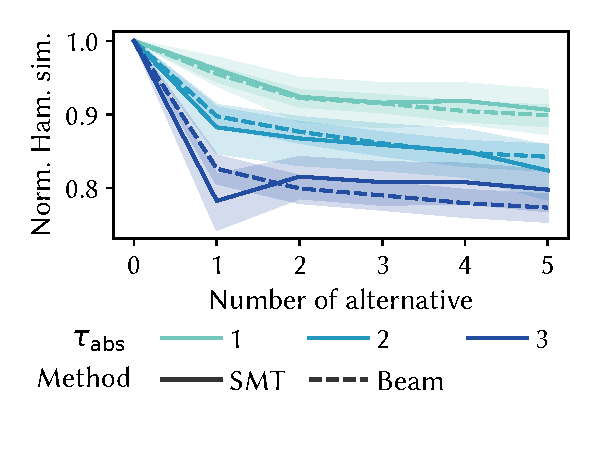
\includegraphics[width=\textwidth, trim=10 25 10 10, clip]{plots/csd-alternatives-hamming.pdf}
		\caption{Normalized Hamming similarity.}
		\label{fig:csd:alternatives-hamming}
	\end{subfigure}
	\hfill
	\begin{subfigure}[t]{0.48\textwidth}
		\centering
		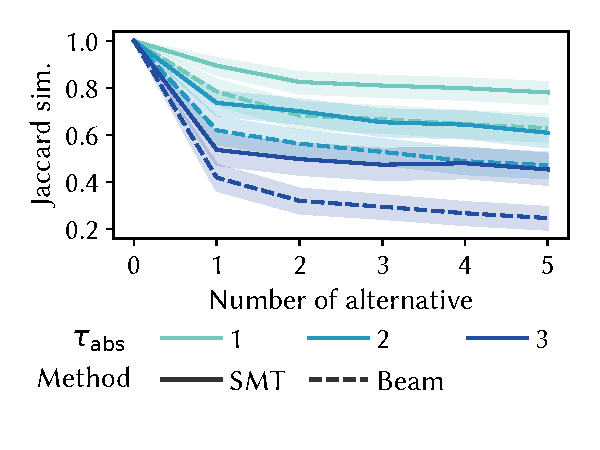
\includegraphics[width=\textwidth, trim=10 25 10 10, clip]{plots/csd-alternatives-jaccard.pdf}
		\caption{Jaccard similarity.}
		\label{fig:csd:alternatives-jaccard}
	\end{subfigure}
	\\ \vspace{\baselineskip}
	\begin{subfigure}[t]{0.48\textwidth}
		\centering
		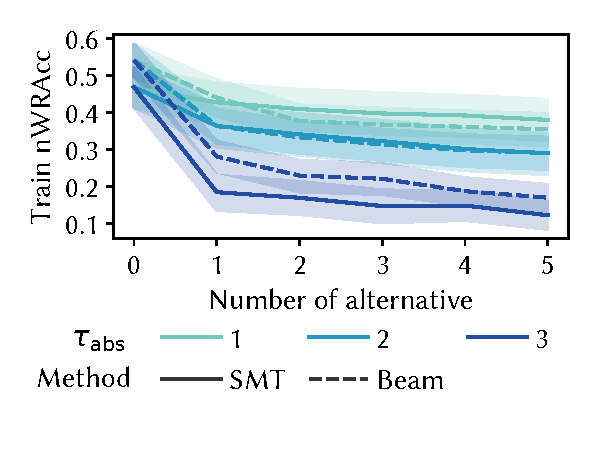
\includegraphics[width=\textwidth, trim=10 25 10 10, clip]{plots/csd-alternatives-train-nwracc.pdf}
		\caption{Training-set subgroup quality (nWRAcc).}
		\label{fig:csd:alternatives-train-nwracc}
	\end{subfigure}
	\hfill
	\begin{subfigure}[t]{0.48\textwidth}
		\centering
		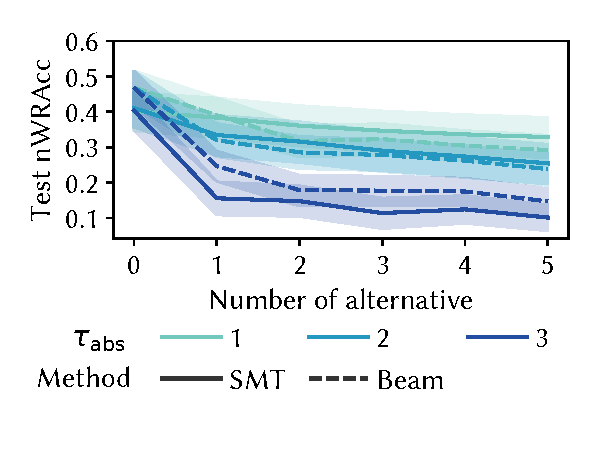
\includegraphics[width=\textwidth, trim=10 25 10 10, clip]{plots/csd-alternatives-test-nwracc.pdf}
		\caption{Test-set subgroup quality (nWRAcc).}
		\label{fig:csd:alternatives-test-nwracc}
	\end{subfigure}
	\caption{
		Mean similarity and quality of alternative subgroup descriptions, with 95\% confidence intervals based on datasets and cross-validation folds, by subgroup-discovery method, number of alternative, and dissimilarity threshold~$\tau_{\text{abs}}$.
	}
	\label{fig:csd:alternatives}
\end{figure}

\paragraph{Subgroup similarity}

Figures~\ref{fig:csd:alternatives-hamming} and~\ref{fig:csd:alternatives-jaccard} visualize the average similarity between the original subgroup and the subgroups induced by alternative subgroup descriptions.
As one would expect, subgroup-membership similarity decreases for more alternatives and the more the subgroup descriptions should differ.
Further, the decrease is strongest from the original subgroup, i.e., the zeroth alternative, to the first alternative but then becomes smaller.
This observation indicates that one may find several alternative subgroup descriptions of comparable similarity to the original one. 
These trends hold for the normalized Hamming similarity (Equation~\ref{eq:csd:hamming-general} and Figure~\ref{fig:csd:alternatives-hamming}) as well as the Jaccard similarity (Equation~\ref{eq:csd:jaccard} and Figure~\ref{fig:csd:alternatives-jaccard}).
The latter yields lower similarity values than the former since it ignores data objects not contained in either of the compared subgroups.

Further, the observed trends exist for the solver-based search method \emph{SMT} as well as the heuristic \emph{Beam}.
\emph{SMT} yields more similar alternative descriptions than \emph{Beam} for the Jaccard similarity, while the normalized Hamming similarity does not show a clear winner.

\paragraph{Subgroup quality}

The average subgroup quality of alternative subgroup descriptions (Figures~\ref{fig:csd:alternatives-train-nwracc} and~\ref{fig:csd:alternatives-test-nwracc}) shows similar trends as subgroup similarity, on the training set as well as on the set test.
In particular, quality also decreases over the dissimilarity threshold~$\tau_{\text{abs}}$ and over the number of alternatives~$a$, with the largest decrease to the first alternative.
For the highest dissimilarity threshold~$\tau_{\text{abs}} = 3$, \emph{Beam} consistently yields higher mean quality than \emph{SMT} for the original subgroup and each alternative.
In contrast, the other two values of~$\tau_{\text{abs}}$ do not clearly favor either subgroup-discovery method.
For both methods, overfitting, measured by the train-test difference in nWRAcc, is lower for the alternative subgroup descriptions than for the original subgroups.
This result may stem from the alternative subgroup descriptions not directly optimizing subgroup quality.

\begin{table}[t]
	\centering
	\caption{
		Mean runtime (in seconds) over datasets and cross-validation folds, by subgroup-discovery method, dissimilarity threshold~$\tau_{\text{abs}}$, and number of alternative.
		Results from the search for alternative subgroup descriptions.
	}
	\begin{tabular}{llrrrrrr}
		\toprule
		\multirow{2}{*}{Method} & \multirow{2}{*}{$\tau_{\text{abs}}$} & \multicolumn{6}{c}{Number of alternative} \\
		\cmidrule(lr){3-8}
		& & 0 & 1 & 2 & 3 & 4 & 5 \\
		\midrule
		\multirow[t]{3}{*}{Beam} & 1 & 12.8 & 8.0 & 7.6 & 7.3 & 7.3 & 7.3 \\
		& 2 & 12.8 & 7.7 & 7.4 & 7.2 & 7.0 & 6.8 \\
		& 3 & 12.8 & 5.8 & 5.1 & 4.7 & 4.1 & 3.5 \\
		\multirow[t]{3}{*}{SMT} & 1 & 1091.7 & 166.0 & 221.5 & 239.6 & 258.1 & 277.9 \\
		& 2 & 1105.2 & 377.5 & 463.5 & 537.5 & 599.4 & 658.3 \\
		& 3 & 1107.4 & 869.1 & 670.8 & 597.6 & 588.1 & 557.6 \\
		\bottomrule
	\end{tabular}
	\label{tab:csd:alteratives-runtime}
\end{table}

\paragraph{Runtime}

Table~\ref{tab:csd:alteratives-runtime} displays the average runtime for searching original and alternative subgroup descriptions.
The search for alternatives is faster for both analyzed subgroup-discovery methods.
\emph{Beam} is generally one to two orders of magnitude faster than \emph{SMT}.
For \emph{Beam}, runtime tends to decrease with an increasing~$\tau_{\text{abs}}$ and number of alternatives, while \emph{SMT} shows a less clear behavior.
In particular, \emph{SMT}'s runtime increases over alternatives for~$\tau_{\text{abs}} \in \{1, 2\}$, i.e., settings that allow reusing features from previous subgroup descriptions.
In contrast, runtime decreases over alternatives for $\tau_{\text{abs}} = k = 3$, which forbids selecting any feature used before.

\subsection{Summary and Discussion}
\label{sec:csd:evaluation:summary-discussion}

\paragraph{Search methods}

The heuristic search methods \emph{Beam} and \emph{BI} were overall best.
These two methods from the literature yielded close-to-optimal quality while being significantly faster than our exhaustive, solver-based search method \emph{SMT}.
They also beat the quality of the exhaustive competitors \emph{BSD} and \emph{SD-Map}, which required discretizing numeric features beforehand.

Setting a solver timeout allows users to control \emph{SMT}'s runtime but results in suboptimal solutions.
\emph{SMT} retains the conceptual advantage that constraints can be added declaratively instead of needing to adapt an algorithmic search procedure to individual constraint types.
For example, besides limiting the selected features, one could easily limit the subgroup size, define secondary quality metrics whose values must pass certain thresholds, or add constraints based on domain knowledge.
The two particular constraint types studied in this article had the advantage of being antimonotonic, which eased their integration into the three evaluated heuristics.

Heuristic solutions were less prone to overfitting than (training-set-)optimal solutions from exhaustive search.
These results highlight the heuristics as serious competitors for any exhaustive search method from the literature, not only our method \emph{SMT}.
Finally, we introduced the novel baseline \emph{MORS}, which provided instantaneous, non-trivial lower bounds for subgroup quality.

\paragraph{Feature-cardinality constraints}

Imposing feature-cardinality constraints sped up the heuristic search methods as well as \emph{BSD} and \emph{SD-Map}, while the picture for the solver-based search method \emph{SMT} was less clear.
Further, this constraint type generally reduced overfitting.
Subgroups using as few as $k=2$ features in their description often yielded already a similar test-set quality as unconstrained subgroups, i.e., using all features.
This result speaks for using small feature sets in subgroup descriptions, which may benefit interpretability for users.

\paragraph{Alternative subgroup descriptions}

Results for alternative subgroup descriptions strongly depended on two parameters, i.e., the number and dissimilarity of alternatives.
With these parameters, users can control alternatives according to their needs.
In general, the difference in quality and similarity between the original subgroup and the first alternative was higher than among the first few alternatives.
In particular, there may be several promising alternatives from which users may choose one based on further criteria.

\paragraph{Problem definition}

As stated in Section~\ref{sec:csd:fundamentals:problem}, we focused on datasets with continuous features and a binary target.
In general, there are also subgroup-discovery methods specifically for categorical data~\cite{herrera2011overview} and other target types~\cite{atzmueller2015subgroup}.
Categorical features can be encoded numerically~\cite{matteucci2023benchmark} and thereby integrated into our formalization and experiments.
Further, the two constraint types we analyzed are independent of the target type.
The chosen binary target is a special case of categorical and numeric targets.
Experimentally, switching the target type would require a different subgroup-quality metric and other datasets.
In our SMT encoding, one would only need to replace the WRAcc objective (Equation~\ref{eq:csd:smt-wracc}) with the new quality metric.
Finally, our baseline \emph{MORS} (Section~\ref{sec:csd:baselines:mors}) would no longer be applicable, though adaptations to other target types may exist.

\section{Related Work}
\label{sec:csd:related-work}

In this section, we review related work.
We cover subgroup discovery in general and the two analyzed constraint types in particular.
Finally, we also discuss adjacent fields.

\paragraph{Subgroup discovery in general}

The terms `subgroup' and `subgroup discovery' have different meanings in different communities, and similar concepts have been reinvented over time.
Our problem definition (Section~\ref{sec:csd:fundamentals:problem}) builds on related work in data mining; see~\cite{atzmueller2015subgroup, helal2016subgroup, herrera2011overview, ventura2018subgroup} for broad surveys of subgroup discovery in this field.
There are also recent works independent from this research~\cite{asudeh2019assessing, lawless2022interpretable, pastor2021looking, sagadeeva2021sliceline}.
These works are only loosely related to ours since their problem definition differs in the optimization objective, type of subgroup description, and employed constraints.

\paragraph{White-box formulations of subgroup discovery}

Nearly all existing subgroup-discovery methods, whether they are exhaustive or heuristic, are problem-specific algorithms.
To our knowledge, optimizing subgroup discovery with a general-purpose SMT solver is novel.
There are only a few white-box formulations for variants of subgroup discovery~\cite{bonates2008maximum, eckstein2002maximum, guns2011itemset, koccak2020exploiting, louveaux2014combinatorial}, which tackle different problem definitions than we do.
E.g., they have additional constraints and neither consider feature-cardinality constraints nor alternative subgroup descriptions.
Further, their experimental evaluations do not compare with existing heuristic subgroup-discovery methods.

\paragraph{Feature-cardinality constraints for subgroup descriptions}

Feature cardinality is a common constraint type~\cite{meeng2021real} and a well-known metric for subgroup complexity~\cite{herrera2011overview}.
However, it is typically integrated into algorithmic rather than solver-based search methods.
\cite{li2015efficient}~formulates a quadratic program to select non-redundant features for subgroup descriptions but only as a subroutine within an algorithmic search.
Also, their optimization problem employs real-valued feature weights as decision variables rather than defining a discrete feature selection.

While several empirical studies use one fixed feature-cardinality threshold for subgroup discovery, only a few studies systematically analyze the impact of different thresholds~\cite{friedman1999bump, lemmerich2010fast, meeng2021real, proencca2022robust}.
They all employ a narrower experimental design than our study does, e.g., compare fewer subgroup-discovery methods.
The broadest of these analyses~\cite{meeng2021real} evaluates three subgroup-discovery methods, including beam and exhaustive search.
However, the study focuses on strategies for discretizing numeric data instead of analyzing feature-cardinality constraints in detail.
The authors compare~$k \in \{1, 2, 3, 4\}$ but not an unconstrained setting.
They use 13 datasets, ten of which have at most ten numeric features, while we employ more and higher-dimensional datasets.

\paragraph{Alternative subgroup descriptions}

To our knowledge, alternative subgroup descriptions in the sense of our article are novel.
Existing approaches for discovering diverse sets of subgroups aim to \emph{minimize} the overlap of contained data objects~\cite{atzmueller2015subgroup, belfodil2019fssd, bosc2018anytime, leeuwen2012diverse, lucas2018ssdp+}, thereby attempting to cover different regions in the dataset.
In contrast, we aim to \emph{maximize} the set similarity of contained data objects to a given subgroup while using different features (Definition~\ref{def:csd:alternative-subgroup-description-discovery}).
Only a few related approaches consider alternatives regarding the subgroup descriptions, which we discuss next.

\cite{leeuwen2012diverse}~proposes six strategies to foster diverse subgroup sets.
Two of these strategies target diverse subgroup descriptions while optimizing subgroup quality.
Both strategies aim at simultaneous rather than sequential search, do not optimize subgroup similarity, and are integrated only into beam search.
Finally, they give users less control than our dissimilarity parameter~$\tau$ does:
One strategy excludes subgroup descriptions that have the same quality and differ in only one condition from an existing subgroup description.
The other uses a global upper bound on how often a feature may be selected in a subgroup set rather than controlling pairwise dissimilarity.

\cite{lopez2023discovering}~introduces the notion of \emph{diverse top-k characteristic lists}, which are sets of lists, each containing multiple patterns, e.g., subgroups.
The same pattern description must not appear in two lists, but any other overlap of descriptions is allowed.
Within lists, patterns should be diverse in terms of data objects covered.

\cite{boley2009non}~introduces the concept of \emph{equivalent subgroup descriptions of minimal length}, which are stricter than alternative subgroup descriptions.
In particular, the former must cover exactly the same set of data objects, like our notion of perfect alternative subgroup descriptions (Definition~\ref{def:csd:perfect-alternative}), instead of maximizing similarity.
Further, a subset of the original feature set must be found instead of using a different feature set under a dissimilarity constraint.
The authors prove $\mathcal{NP}$-hardness, on which our complexity proof for perfect-subgroup discovery (Proposition~\ref{prop:csd:complexity-cardinality-np-perfect-subgroup}) builds.
Additionally, they propose two search algorithms but do not pursue a solver-based search.

\emph{Redescription mining} aims to find pairs or sets of descriptions that cover exactly or approximately the same data objects~\cite{galbrun2017redescription, ramakrishnan2004turning}.
Our notion of alternative subgroup descriptions pursues a similar goal.
However, the search for redescriptions is simultaneous and unsupervised~\cite{ramakrishnan2004turning}, while we search alternatives sequentially and start with an original subgroup found supervised, i.e., optimizing subgroup quality.
Further, the dissimilarity criteria for redescriptions differ from ours, e.g., having features pre-partitioned into non-overlapping sets~\cite{galbrun2017redescription, gallo2008finding, mihelcic2023complexity} or
requiring only one arbitrary part of the description to differ~\cite{parida2005redescription}, while we give users control with the dissimilarity threshold~$\tau$.
Also, redescriptions may use more complex patterns than subgroup descriptions, e.g., more logical operators than only AND ($\land$) to combine conditions over features.

\paragraph{Further related work}

There are white-box formulations for various classification models like decision trees, decision sets, and decision lists~\cite{ignatiev2021reasoning, narodytska2018learning, shati2021sat, yu2021learning}.
These models also use conjunctions of conditions to form descriptive rules, but they try to describe the dataset globally instead of focusing on individual interesting regions like subgroups.

Considering constraints in data mining is a general theme beyond subgroup discovery; see~\cite{grossi2017survey} for a survey.
Similarly, finding alternative or diverse solutions is a concern in various fields, e.g., clustering~\cite{bailey2014alternative}, subspace search~\cite{fouche2021efficient}, and explainable-AI paradigms like counterfactuals~\cite{guidotti2022counterfactual}, criticisms~\cite{kim2016examples}, and semifactuals~\cite{artelt2022even}.
Generally, these fields have considerably different problem definitions than subgroup discovery, so we only discuss two examples shortly:

(1)  In the field of feature selection, \cite{bach2023finding, bach2024alternative} propose a white-box formulation of finding alternative feature sets.
However, traditional feature selection differs from subgroup discovery by `only' selecting the features, which are then used by a prediction model, instead of directly determining bounds on feature values to define a model.

(2) \cite{karimi2020model, mohammadi2021scaling, mothilal2020explaining, russell2019efficient} propose approaches for diverse counterfactual explanations.
Counterfactuals are data objects that are as similar as possible to a given data object but with a different prediction of a given classifier.
In contrast, alternative subgroup descriptions aim at similar predictions for all data objects but a different feature selection.

\section{Conclusion}
\label{sec:csd:conclusion}

Subgroup-discovery methods constitute an important category of interpretable machine-learning models.
This study investigated two constraint types for subgroup discovery: 
on the number of selected features and for alternative subgroup descriptions.
We proved $\mathcal{NP}$-completeness for the corresponding optimization problems.
We also studied integrating these constraint types into a novel SMT formulation of subgroup discovery and existing heuristic search methods.
Finally, we conducted experiments with eight subgroup-discovery methods and 27 binary-classification datasets.
Overall, two heuristic search methods provided the best combination of runtime and subgroup quality, while the performance of exhaustive search methods was unsatisfactory.

Future work could apply our domain-independent methods to specific use cases and interpret the resulting subgroup descriptions qualitatively, i.e., from the domain perspective.

\begin{acks}
We want to thank Klemens Böhm for feedback on an earlier version of this article.
\end{acks}

\bibliographystyle{ACM-Reference-Format}
\bibliography{references}

%\appendix % unused in current version

\end{document}
\endinput
